% ======================================================================
% MONOGRAFIA — SISTEMA DE AUTOMAÇÃO E SUPERVISÃO PARA ESPECIAÇÃO DE Hg
% Classe: memoir + formatação manual ABNT (sem abntex2 no ambiente).
% Compilar: pdflatex -> bibtex -> pdflatex -> pdflatex (ver build.sh)
% ======================================================================
\documentclass[12pt,a4paper,openright,oneside]{memoir}

% ----------------------------- pacotes básicos ------------------------
\usepackage[T1]{fontenc}
\usepackage[utf8]{inputenc}
\usepackage[brazilian]{babel}
\shorthandoff{"}          % desativa shorthand " do babel brazilian
\usepackage{mathptmx}     % fonte Times (texto + matemática)
\usepackage[a4paper,top=3cm,bottom=2cm,left=3cm,right=2cm]{geometry}
\usepackage{amsmath,amssymb}
\usepackage{graphicx}
\graphicspath{{figures/}}
\usepackage[table]{xcolor}
\usepackage{booktabs}
\usepackage{longtable}
\usepackage{caption}
\usepackage{enumitem}
\usepackage{url}
\usepackage{tikz}
\usetikzlibrary{arrows.meta,positioning,shapes.geometric,calc}
\usepackage[pdftex,bookmarks=true,colorlinks=true,linkcolor=black,
            citecolor=black,urlcolor=black,hypertexnames=false]{hyperref}

% ------------------------- comandos auxiliares ------------------------
\newcommand{\celsius}{\ensuremath{^{\circ}\mathrm{C}}}
\newcommand{\graus}[1]{\ensuremath{#1^{\circ}}}
\newcommand{\daq}{DAQ}
\newcommand{\ihm}{IHM}
\newcommand{\pid}{PID}

% ----------------------------- espaçamento ----------------------------
\OnehalfSpacing
\setlength{\parindent}{1.25cm}
\setlength{\parskip}{0pt}

% --------------------------- estilo de capítulo -----------------------
\makechapterstyle{monografia}{%
  \renewcommand{\chapnamefont}{\normalfont\bfseries}%
  \renewcommand{\chapnumfont}{\normalfont\Large\bfseries}%
  \renewcommand{\chaptitlefont}{\normalfont\Large\bfseries}%
  \setlength{\beforechapskip}{0.3\baselineskip}%
  \setlength{\midchapskip}{0.5\baselineskip}%
  \setlength{\afterchapskip}{1.5\baselineskip}%
  \renewcommand{\printchaptername}{}%
  \renewcommand{\chapternamenum}{}%
}
\chapterstyle{monografia}
\setsecnumdepth{subsubsection}
\settocdepth{subsection}

% Título de seções: caixa alta para nível primário (ABNT NBR 14724)
\renewcommand{\thesection}{\arabic{chapter}.\arabic{section}}
\renewcommand{\thesubsection}{\thesection.\arabic{subsection}}
\renewcommand{\thesubsubsection}{\thesubsection.\arabic{subsubsection}}
\setsecheadstyle{\normalfont\bfseries\MakeUppercase}
\setsubsecheadstyle{\normalfont\bfseries}
\setsubsubsecheadstyle{\normalfont\bfseries\itshape}

% ------------------------ cabeçalho/rodapé ----------------------------
\pagestyle{plain}
\nouppercaseheads

% --------------------- legendas de figuras e tabelas ------------------
\captionsetup{font=small,labelfont=bf,textfont=bf,labelsep=endash}
\renewcommand{\figurename}{Figura}
\renewcommand{\tablename}{Tabela}

% ------------------------- numeração de equação -----------------------
\numberwithin{equation}{chapter}

% ------------------ dados institucionais (preencher) ------------------
\newcommand{\instituicao}{Instituto Federal Fluminense}
\newcommand{\curso}{[CURSO]}
\newcommand{\titulocurso}{Aprendizes da vida}
\newcommand{\autor}{William da Silva Vianna\\ Renato Gomes Sobral Barcellos}
\newcommand{\orientador}{Os pr\'oprios autores}
\newcommand{\cidade}{Campos dos Goytacazes}
\newcommand{\ano}{2026}

% ======================================================================
\begin{document}

% ----------------------------------------------------------------------
% CAPA
% ----------------------------------------------------------------------
\thispagestyle{empty}
\begin{center}
\MakeUppercase{\instituicao}\\[0.3cm]
\MakeUppercase{\curso}\\[4.5cm]
{\large \autor}\\[4.0cm]
{\Large \bfseries
  DESENVOLVIMENTO DE SISTEMA DE AUTOMAÇÃO E SUPERVISÃO PARA
  PREPARAÇÃO DE AMOSTRAS EM ESPECIAÇÃO DE MERCÚRIO}\\[5.5cm]
{\large \cidade}\\[0.2cm]
{\large \ano}
\end{center}
\clearpage

% ----------------------------------------------------------------------
% FOLHA DE ROSTO
% ----------------------------------------------------------------------
\thispagestyle{empty}
\begin{center}
{\large \autor}\\[5.0cm]
{\Large \bfseries
  DESENVOLVIMENTO DE SISTEMA DE AUTOMAÇÃO E SUPERVISÃO PARA
  PREPARAÇÃO DE AMOSTRAS EM ESPECIAÇÃO DE MERCÚRIO}
\end{center}
\vspace{3.0cm}
\begin{center}
\begin{minipage}[t]{9.0cm}
Monografia apresentada ao curso de \curso{} da \instituicao{}
como requisito parcial para a obtenção do título de
\titulocurso{}.
\end{minipage}
\end{center}
\vspace{1.0cm}
\begin{center}
\begin{minipage}[t]{9.0cm}
Orientador: \orientador{}
\end{minipage}
\end{center}
\vfill
\begin{center}
{\large \cidade}\\[0.2cm]
{\large \ano}
\end{center}
\clearpage

% ----------------------------------------------------------------------
% FRENTE PRÉ-TEXTUAL (numeração romana)
% ----------------------------------------------------------------------
\frontmatter
\pagestyle{plain}

% ------------------------------ dedicatória ---------------------------
\chapter*{Dedicatória}
\addcontentsline{toc}{chapter}{Dedicatória}
\begin{flushright}
\textit{[Dedicatória — texto opcional a ser redigido pelo autor.]}
\end{flushright}
\clearpage

% ---------------------------- agradecimentos --------------------------
\chapter*{Agradecimentos}
\addcontentsline{toc}{chapter}{Agradecimentos}
\textit{[Agradecimentos — texto opcional a ser redigido pelo autor,
mencionando orientador(a), instituição e demais pessoas que
contribuíram para o trabalho.]}
\clearpage

% ------------------------------- epígrafe -----------------------------
\chapter*{Epígrafe}
\addcontentsline{toc}{chapter}{Epígrafe}
\begin{flushright}
\textit{[Epígrafe — citação opcional escolhida pelo autor.]}
\end{flushright}
\clearpage

% ------------------------------- resumo -------------------------------
\chapter*{RESUMO}
\addcontentsline{toc}{chapter}{RESUMO}
% Resumo em português
A especiação de mercúrio é uma técnica analítica utilizada para identificar e
quantificar as diferentes espécies químicas desse elemento em amostras
ambientais, tais como mercúrio elementar (Hg$^0$) e metilmercúrio. O
procedimento de preparação de amostras exige o controle rigoroso de uma
sequência de etapas químicas --- derivatização com tetraetilborato de sódio,
criofocalização em nitrogênio líquido a aproximadamente $-196\,\celsius$,
aquecimento controlado do Tubo U até $230\,\celsius$ e atomização a
$700\,\celsius$ ---, de modo que a qualidade da rampa de temperatura imposta ao
Tubo U determina diretamente a correta separação e identificação das espécies.

Este trabalho apresenta o projeto e a implementação de um sistema de automação e
supervisão para a preparação de amostras em especiação de mercúrio, concebido
para substituir um sistema legado baseado em LabVIEW. O sistema adota uma
arquitetura mestre-escravo composta por um Raspberry Pi, que executa a lógica de
alto nível em Python (máquina de estados finita, controle proporcional-integral-
derivativo --- PID --- e persistência de parâmetros), um Arduino Uno operando
como módulo de aquisição de dados em tempo real, responsável pelo acionamento de
válvulas e fornos, pela leitura de termopares via interface SPI e por um
watchdog de segurança, e uma interface homem-máquina (IHM) Web desenvolvida em
React e TypeScript, com monitoramento em tempo real via WebSocket, Diagrama de
Tempos, gráficos de tendência e modos automático e manual.

O processo foi modelado em uma máquina de estados finita com quatro fases de
acionamento ($T_0$ a $T_3$) e uma matriz de atuadores (válvulas SV1 a SV5,
bomba peristáltica e fornos). O controle de temperatura emprega uma estratégia
PID mista: abaixo de $0\,\celsius$, a variável manipulada é calculada pela razão
entre a taxa de aquecimento desejada pelo operador e a taxa do sistema,
enquanto, acima desse limiar, um controlador PID em malha fechada segue um
setpoint dinâmico de rampa até $230\,\celsius$; o Forno 2 é regulado em setpoint
fixo de $700\,\celsius$. A comunicação entre o Raspberry Pi e o Arduino é
realizada por pacotes JSON em enlace serial a 4 Hz, com handshake de
parametrização e watchdog duplo que impõe o retorno ao estado seguro em caso de
perda de comunicação.

O desenvolvimento seguiu a abordagem de desenvolvimento orientado a testes, com
validação por testes unitários, de integração, funcionais e de segurança
executados em ambiente de simulação sem hardware físico. Os resultados mostram
que a arquitetura proposta atende aos requisitos funcionais e de segurança
definidos, garantindo repetibilidade da lógica de controle, persistência
auditável dos parâmetros do método e parada segura automática diante de falhas
de comunicação. A validação em bancada, com a calibração da curva de aquecimento
do Tubo U e a verificação experimental da rampa de temperatura, é apresentada
como etapa de continuidade do trabalho.

\vspace{0.5cm}
\noindent\textbf{Palavras-chave:} automação; controle PID; especiação de
mercúrio; máquina de estados finita; interface homem-máquina; sistema embarcado.

\clearpage

% ------------------------------- abstract -----------------------------
\chapter*{ABSTRACT}
\addcontentsline{toc}{chapter}{ABSTRACT}
% Abstract em inglês
Mercury speciation is an analytical technique used to identify and quantify the
different chemical species of this element in environmental samples, such as
elemental mercury (Hg$^0$) and methylmercury. The sample preparation procedure
requires strict control of a sequence of chemical steps --- derivatization with
sodium tetraethylborate, cryofocusing in liquid nitrogen at approximately
$-196\,\celsius$, controlled heating of the U-tube up to $230\,\celsius$, and
atomization at $700\,\celsius$ --- so that the quality of the temperature ramp
applied to the U-tube directly determines the correct separation and
identification of the species.

This work presents the design and implementation of an automation and
supervision system for sample preparation in mercury speciation, conceived to
replace a legacy LabVIEW-based system. The system adopts a master-slave
architecture composed of a Raspberry Pi running the high-level logic in Python
(finite state machine, proportional-integral-derivative --- PID --- control and
parameter persistence), an Arduino Uno operating as a real-time data
acquisition module responsible for driving valves and furnaces, reading
thermocouples through the SPI interface and running a safety watchdog, and a
Web human-machine interface (HMI) developed in React and TypeScript, with
real-time monitoring over WebSocket, a timing diagram, trend charts and
automatic and manual modes.

The process was modeled as a finite state machine with four actuation phases
($T_0$ to $T_3$) and an actuator matrix (solenoid valves SV1 to SV5,
peristaltic pump and furnaces). Temperature control employs a mixed PID
strategy: below $0\,\celsius$, the manipulated variable is computed as the ratio
between the operator-required heating rate and the system rate, whereas above
this threshold a closed-loop PID controller tracks a dynamic ramp setpoint up to
$230\,\celsius$; Furnace 2 is regulated at a fixed setpoint of $700\,\celsius$.
Communication between the Raspberry Pi and the Arduino is carried out through
JSON packets over a serial link at 4~Hz, with a parametrization handshake and a
double watchdog that forces the return to the safe state in case of
communication loss.

The development followed a test-driven approach, validated by unit,
integration, functional and safety tests executed in a simulation environment
without physical hardware. The results show that the proposed architecture
meets the defined functional and safety requirements, ensuring repeatability of
the control logic, auditable persistence of the method parameters and automatic
safe shutdown in the presence of communication failures. Bench validation, with
the calibration of the U-tube heating curve and the experimental verification of
the temperature ramp, is presented as a follow-up stage of this work.

\vspace{0.5cm}
\noindent\textbf{Keywords:} automation; PID control; mercury speciation;
finite state machine; human-machine interface; embedded system.

\clearpage

% ------------------------- lista de figuras ---------------------------
\renewcommand{\listfigurename}{LISTA DE FIGURAS}
\listoffigures*
\clearpage

% ------------------------- lista de tabelas ---------------------------
\renewcommand{\listtablename}{LISTA DE TABELAS}
\listoftables*
\clearpage

% --------------------- lista de abreviaturas e siglas ----------------
\chapter*{LISTA DE ABREVIATURAS E SIGLAS}
\addcontentsline{toc}{chapter}{LISTA DE ABREVIATURAS E SIGLAS}
\begin{tabular}{@{}p{3.6cm}p{11.6cm}@{}}
AAS   & Espectrometria de absorção atômica (Atomic Absorption Spectrometry)\\
AFS   & Espectrometria de fluorescência atômica (Atomic Fluorescence Spectrometry)\\
API   & Interface de programação de aplicações\\
CVAAS & Absorção atômica com vapor frio (Cold Vapor AAS)\\
\daq{}   & Aquisição de dados (Data Acquisition)\\
FSM   & Máquina de estados finita (Finite State Machine)\\
GC    & Cromatografia gasosa\\
Hg    & Mercúrio\\
HTTP  & Protocolo de transferência de hipertexto\\
\ihm{}   & Interface homem-máquina\\
JSON  & JavaScript Object Notation\\
LSB   & Bit menos significativo\\
MISO  & Master In Slave Out (SPI)\\
MOSI  & Master Out Slave In (SPI)\\
N$_2$  & Nitrogênio molecular (nitrogênio líquido)\\
\pid{}   & Controlador proporcional-integral-derivativo\\
PWM   & Modulação por largura de pulso (Pulse Width Modulation)\\
RPi   & Raspberry Pi\\
REST  & Representational State Transfer\\
SP    & Setpoint (valor de referência)\\
SPI   & Serial Peripheral Interface\\
SSR   & Relé de estado sólido\\
SV    & Válvula solenóide\\
TEBS  & Tetraetilborato de sódio (NaBEt$_4$)\\
VM    & Variável manipulada\\
VP    & Variável de processo\\
WS    & WebSocket\\
\end{tabular}
\clearpage

% ----------------------------- lista de símbolos ----------------------
\chapter*{LISTA DE SÍMBOLOS}
\addcontentsline{toc}{chapter}{LISTA DE SÍMBOLOS}
\begin{tabular}{@{}p{4.2cm}p{11cm}@{}}
$K_p$    & Ganho proporcional do controlador\\
$T_i$    & Tempo integral do controlador (min)\\
$T_d$    & Tempo derivativo do controlador (min)\\
$e(t)$   & Sinal de erro (diferença entre setpoint e variável de processo)\\
$u(t)$   & Variável manipulada (saída do controlador)\\
$T_0,\dots,T_3$ & Tempos de acionamento do ciclo de preparação\\
$t_1,t_2,t_3$   & Durações configuráveis das fases (s)\\
$VM_u$, $VM_{f2}$ & Variável manipulada do Tubo U e do Forno 2 (PWM 0--255)\\
$\dot{T}$ & Taxa de aquecimento ($^{\circ}$C/s)\\
\end{tabular}
\clearpage

% ------------------------------- sumário ------------------------------
\renewcommand{\contentsname}{SUMÁRIO}
\tableofcontents*
\clearpage

% ======================================================================
% CORPO PRINCIPAL (numeração arábica)
% ======================================================================
\mainmatter
% ======================================================================
% CAPÍTULO 1 — INTRODUÇÃO
% ======================================================================
\chapter{INTRODUÇÃO}

\section{Contextualização do tema}

O mercúrio (Hg) é um poluente global de elevada toxicidade que pode ser
liberado para o ambiente por fontes naturais e antropogênicas. Seu
comportamento, transporte e risco toxicológico dependem fortemente da espécie
química em que se encontra: o metilmercúrio, por exemplo, é uma forma
neurotóxica que se acumula na cadeia alimentar, enquanto o mercúrio elementar
apresenta elevada pressão de vapor e grande mobilidade atmosférica. Nesse
contexto, a \emph{especiação} de mercúrio --- isto é, a determinação das
diferentes formas químicas do elemento em uma amostra --- é indispensável para
avaliações de risco e estudos biogeoquímicos confiáveis \cite{leermakers2005,
bloom1989}.

A determinação de espécies de mercúrio exige um procedimento analítico de
preparação de amostras composto por etapas sequenciais bem definidas. No sistema
considerado neste trabalho, a amostra líquida é submetida à \emph{derivatização}
com tetraetilborato de sódio (TEBS, NaBEt$_4$), que volatiliza as espécies de
mercúrio presentes. Em seguida, um gás de arraste (hélio) conduz os vapores até
um Tubo U imerso em um copo com nitrogênio líquido, onde ocorre a
\emph{criofocalização} das espécies a aproximadamente $-196\,\celsius$. Após o
período definido pelo operador, o copo é abaixado, o aquecimento do Tubo U é
iniciado e as espécies são liberadas progressivamente conforme sua temperatura
de volatilização, sendo então atomizadas a $700\,\celsius$ em um segundo forno e
detectadas por espectrometria de absorção atômica.

A qualidade analítica do processo depende diretamente da forma como a
temperatura do Tubo U é controlada ao longo do tempo: idealmente, uma rampa
linear de temperatura na faixa de aproximadamente $-50\,\celsius$ a
$230\,\celsius$ permite correlacionar o instante de liberação de cada espécie
com sua temperatura de volatilização. Qualquer não linearidade na rampa
compromete a separação das espécies e produz picos sobrepostos no detector,
invalidando a análise. O processo físico completo é detalhado no Capítulo~2, e
os requisitos técnicos que o especificam estão documentados nos arquivos de
requisitos e de especificação do sistema.

\section{Problema de pesquisa}

O equipamento de preparação de amostras descrito era originalmente controlado
por um sistema supervisório desenvolvido em LabVIEW, executado em um computador
com comunicação serial a um módulo de aquisição de dados (Arduino Uno). Com o
tempo, esse sistema legado passou a apresentar limitações relevantes, que podem
ser agrupadas em cinco frentes principais:

\begin{enumerate}[label=\roman*)]
  \item \textbf{Controle inadequado da rampa de temperatura do Tubo U.} O
  sistema não garante a linearidade da rampa na faixa de $-50\,\celsius$ a
  $230\,\celsius$, comprometendo a separação e a identificação das espécies de
  mercúrio e resultando em picos sobrepostos, análises inválidas e retrabalho;
  \item \textbf{Parâmetros não persistentes e pouco rastreáveis.} Os ganhos dos
  controladores e os tempos do método ficavam fixos ou sem persistência
  confiável entre execuções, prejudicando a repetibilidade e a auditoria do
  método;
  \item \textbf{Interface propensa a erro humano.} A interface legada não
  dispunha de um sinótico claro do processo, de indicadores de tendência ou de
  uma parada de emergência centralizada de alta prioridade;
  \item \textbf{Acoplamento entre a lógica de aplicação e a execução em tempo
  real.} A ausência de separação entre o supervisório e a aquisição de campo
  dificultava a depuração, a manutenção e a evolução do sistema;
  \item \textbf{Segurança insuficiente.} Não havia um mecanismo de watchdog que
  desligasse os aquecedores automaticamente em caso de perda de comunicação,
  expondo o equipamento ao risco de congelamento permanente do Tubo U ou de
  sobreaquecimento dos fornos.
\end{enumerate}

A partir desse diagnóstico, o problema de pesquisa pode ser enunciado da
seguinte forma: \emph{como projetar e implementar um sistema de automação e
supervisão que garanta o controle preciso e seguro do processo de preparação de
amostras em especiação de mercúrio, superando as limitações do sistema legado e
preservando a repetibilidade analítica do método?}

\section{Justificativa}

A substituição do sistema legado é motivada, em primeiro lugar, pela necessidade
de \emph{repetibilidade analítica comprovável}. Métodos de especiação dependem
da reprodutibilidade da rampa de temperatura e da estabilidade das condições do
processo; a persistência dos parâmetros do método e o registro de tendências
permitem auditoria e rastreabilidade das análises. Em segundo lugar, a
modernização apoia-se na disponibilidade de plataformas de baixo custo e alta
confiabilidade --- como o Raspberry Pi e o Arduino Uno --- capazes de atender
aos requisitos de tempo real e de interface do processo a um custo muito menor
que soluções baseadas em controladores lógicos programáveis industriais ou em
licenças proprietárias de software de supervisão \cite{arduino, raspberrypi}.

Em terceiro lugar, a dimensão de \emph{segurança operacional} é crítica em um
ambiente laboratorial que manipula nitrogênio líquido e aquecedores de alta
temperatura. A ausência de uma parada segura automática representa risco de dano
ao equipamento --- como o congelamento permanente do Tubo U --- e à amostra.
Por fim, do ponto de vista acadêmico, o trabalho integra conceitos de controle
de processos, sistemas embarcados, comunicação industrial, engenharia de
software e interface homem-máquina, constituindo um estudo de caso aplicado de
engenharia de automação.

\section{Objetivos}

\subsection{Objetivo geral}

Projetar e implementar um sistema de automação e supervisão para a preparação de
amostras em especiação de mercúrio, baseado em máquina de estados finita,
controle PID misto, módulo de aquisição de dados em tempo real e interface
homem-máquina Web, com parâmetros persistentes e segurança operacional.

\subsection{Objetivos específicos}

\begin{enumerate}[label=\arabic*)]
  \item Modelar o processo de preparação de amostras (fases $T_0$ a $T_3$) em
  uma máquina de estados finita com matriz de acionamento dos atuadores (SV1 a
  SV5, bomba e fornos);
  \item Implementar o controle PID misto do Forno 1 (Tubo U) --- razão de taxas
  de aquecimento para temperaturas abaixo de $0\,\celsius$ e controle PID em
  malha fechada acima desse limiar --- e o controle do Forno 2 (atomizador) em
  setpoint fixo de $700\,\celsius$;
  \item Definir e implementar o protocolo de comunicação JSON estruturado entre
  o Raspberry Pi e o Arduino, operando em ciclo de controle de 4~Hz, com
  handshake de parametrização e pacotes de escrita e de leitura;
  \item Desenvolver o firmware do módulo de aquisição de dados no Arduino Uno,
  responsável pelo acionamento dos atuadores, pela leitura de termopares via
  SPI e pelo watchdog de segurança;
  \item Desenvolver uma IHM Web (React e TypeScript) com monitoramento em tempo
  real, Diagrama de Tempos, gráficos de tendência e painéis de controle e de
  configuração;
  \item Implementar a persistência atômica dos parâmetros do método em arquivo
  JSON, com backup rotativo e validação de faixas;
  \item Validar o sistema por meio de testes unitários, de integração,
  funcionais e de segurança, seguindo a estratégia de desenvolvimento orientado
  a testes adotada no projeto.
\end{enumerate}

\section{Hipótese}

A hipótese de trabalho é que uma arquitetura mestre-escravo composta por um
Raspberry Pi executando a lógica de supervisão e controle em Python e um Arduino
Uno atuando como DAQ em tempo real, integrados por um protocolo JSON a 4~Hz e
supervisionados por uma IHM Web, é capaz de atender aos requisitos funcionais e
de segurança do processo de preparação de amostras, proporcionando controle
preciso da rampa de temperatura, persistência auditável dos parâmetros e parada
segura automática diante de falhas de comunicação, com custo e flexibilidade
superiores aos do sistema legado.

\section{Delimitação do trabalho}

O escopo deste trabalho limita-se à modernização do software de automação e
supervisão do processo de preparação de amostras (versão V1), conforme definido
na documentação de requisitos do sistema. Não fazem parte do
escopo: a integração automática com o detector Lumex (apenas a indicação do
início de leitura é considerada), a calibração automática dos termopares, o
controle de vazão dos rotâmetros (regulagem manual) e mecanismos de
autenticação multiusuário, previstos para versões futuras. A validação
experimental em bancada com o processo físico, incluindo a calibração da curva
de aquecimento do Tubo U e a verificação da linearidade da rampa, é tratada como
etapa de continuidade, sendo o presente desenvolvimento validado em ambiente de
simulação por meio de testes automatizados.

\section{Visão geral da metodologia}

Do ponto de vista metodológico, o trabalho caracteriza-se como uma pesquisa
aplicada, de natureza experimental e abordagem quantitativa, organizada segundo
as etapas de: (i) levantamento e análise dos requisitos do processo a partir da
documentação técnica existente; (ii) definição da arquitetura do sistema; (iii)
desenvolvimento incremental do firmware, do backend e da IHM Web; e (iv)
validação por testes automatizados. O desenvolvimento seguiu práticas de
especificação dirigida e de desenvolvimento orientado a testes, em que os
contratos de interface e os critérios de aceitação foram definidos antes da
implementação \cite{beck2002}. O detalhamento metodológico é
apresentado no Capítulo~4.

\section{Estrutura da monografia}

Este trabalho está organizado em sete capítulos. O Capítulo~1 (presente)
contextualiza o tema e apresenta o problema, a justificativa e os objetivos. O
Capítulo~2 desenvolve a fundamentação teórica, abordando a química do processo,
os conceitos de controle e a base tecnológica empregada. O Capítulo~3 apresenta
os trabalhos relacionados e o posicionamento da solução proposta. O Capítulo~4
descreve a metodologia adotada. O Capítulo~5 detalha o desenvolvimento do
sistema, desde a arquitetura até a implementação de cada módulo. O Capítulo~6
apresenta os experimentos e os resultados obtidos na validação, com a respectiva
discussão. Por fim, o Capítulo~7 apresenta as conclusões e as sugestões para
trabalhos futuros.

% ======================================================================
% CAPÍTULO 2 — FUNDAMENTAÇÃO TEÓRICA
% ======================================================================
\chapter{FUNDAMENTAÇÃO TEÓRICA}

Este capítulo apresenta os conceitos necessários à compreensão do problema e da
solução desenvolvida. Inicialmente, aborda-se a química e o processo de
especiação de mercúrio; em seguida, os fundamentos de automação e controle de
processos, incluindo o controlador PID e as máquinas de estado finitas; depois,
a base tecnológica de sistemas embarcados e comunicação; e, por fim, os
elementos de interface homem-máquina e de segurança funcional empregados.

\section{Especiação de mercúrio}

O mercúrio é um elemento traço de interesse ambiental e sanitário reconhecido
por sua toxicidade e por sua capacidade de ser transportado a longas distâncias
na atmosfera. Do ponto de vista analítico, porém, a determinação do teor total
de mercúrio em uma amostra é insuficiente para avaliações de risco: as espécies
de mercúrio apresentam toxicidades e comportamentos biogeoquímicos distintos, e
é a \emph{especiação} --- a determinação das concentrações das diferentes formas
químicas --- que fornece a informação relevante \cite{leermakers2005}.

As espécies de interesse mais frequentes em amostras ambientais são o mercúrio
elementar (Hg$^0$) e o metilmercúrio (CH$_3$Hg$^+$), além de outras formas
orgânicas e inorgânicas. Devido às baixíssimas concentrações típicas (da ordem
de picogramas a nanogramas), as determinações exigem etapas de derivação
química que convertam as espécies em formas voláteis e estáveis, adequadas à
separação e à detecção \cite{bloom1989, leermakers2005}.

\section{O processo de preparação de amostras}

O sistema considerado neste trabalho executa a etapa de \emph{preparação de
amostras} que antecede a detecção propriamente dita. A Figura~\ref{fig:processo}
apresenta, de forma esquemática, os principais componentes do processo: o frasco
de reação contendo a amostra, o dissecante de náfion, o Tubo U com o copo de
nitrogênio líquido, o Forno 2 e o detector.

\begin{figure}[htbp]
\centering
\begin{tikzpicture}[
  scale=0.82, transform shape,
  font=\small,
  block/.style={rectangle, draw, minimum width=2.2cm, minimum height=0.8cm,
                align=center},
  arr/.style={-{Latex[length=2mm]}, thick}
]
  \node[block] (fr) at (0,0) {Frasco de rea\c{c}\~ao};
  \node[block] (na) at (4.2,0) {Dissecante\\ (n\'afion)};
  \node[block] (tu) at (8.4,0) {Tubo U\\ (Forno 1)};
  \node[block] (f2) at (11.6,0) {Forno 2\\ (atomizador)};
  \node[block] (lu) at (14.8,0) {Detector\\ Lumex};
  \node[rectangle, draw, dashed, minimum width=2.6cm, minimum height=1.0cm,
        align=center] (cop) at (8.4,-2.0) {Copo de N$_2$\\ $-196\,\celsius$};
  \draw[arr] (fr) -- node[above,font=\scriptsize]{h\'elio + vapor} (na);
  \draw[arr] (na) -- node[above,font=\scriptsize]{esp\'ecies} (tu);
  \draw[arr] (tu) -- (f2);
  \draw[arr] (f2) -- (lu);
  \draw[arr,<->] (cop) -- (tu);
\end{tikzpicture}
\caption{Representa\c{c}\~ao esquem\'atica do processo de prepara\c{c}\~ao de amostras.}
\label{fig:processo}
\par\vspace{2pt}{\footnotesize Fonte: elaborada pelo autor com base na documenta\c{c}\~ao t\'ecnica do projeto.}
\end{figure}

\subsection{Derivatiza\c{c}\~ao}

A amostra l\'iquida \'e inserida no frasco de rea\c{c}\~ao, onde recebe uma
solu\c{c}\~ao de tetraetilborato de s\'odio (TEBS, NaBEt$_4$). O TEBS promove a
\emph{derivatiza\c{c}\~ao} das esp\'ecies de merc\'urio, convertendo-as em
formas alquiladas vol\'ateis e termicamente est\'aveis. Esse procedimento de
etila\c{c}\~ao em fase aquosa, seguido de cromatografia gasosa e detec\c{c}\~ao
por fluoresc\^encia at\^omica com vapor frio, \'e uma das t\'ecnicas cl\'assicas
de especia\c{c}\~ao de merc\'urio \cite{bloom1989, liang1994}. O g\'as h\'elio,
inerte e de elevada pureza, \'e introduzido no frasco com duas finalidades:
agitar a amostra e arrastar (purgar) os vapores das esp\'ecies derivatizadas em
dire\c{c}\~ao \`as pr\'oximas etapas do sistema.

\subsection{Secagem e criofocaliza\c{c}\~ao}

Ao purgar os vapores, o h\'elio carrega consigo umidade da solu\c{c}\~ao, que
constitui um interferente para a criofocaliza\c{c}\~ao e para a medi\c{c}\~ao.
Um dissecante de \emph{n\'afion} --- uma membrana polim\'erica perme\'avel
seletivamente \`a \'agua --- \'e empregado para remover a umidade do fluxo
gasoso antes de este atingir o Tubo U.

O Tubo U \'e um tubo de vidro em forma de ``U'' envolvido por um filamento
resistivo (o Forno 1). O tubo est\'a imerso em um copo contendo nitrog\^enio
l\'iquido a aproximadamente $-196\,\celsius$, mantido suspenso por um pist\~ao
criog\^enico (v\'alvula SV5). Nessa temperatura, as esp\'ecies derivatizadas que
chegam pelo fluxo de h\'elio s\~ao retidas por \emph{criofocaliza\c{c}\~ao},
concentrando-se em uma zona estreita do tubo, o que melhora a resolu\c{c}\~ao da
posterior libera\c{c}\~ao t\'ermica.

\subsection{Rampa de temperatura e separa\c{c}\~ao das esp\'ecies}

Ap\'os o per\'iodo de criofocaliza\c{c}\~ao, definido pelo operador, o copo de
nitrog\^enio \'e abaixado e o aquecimento do Forno 1 \'e iniciado. A temperatura
do Tubo U deve crescer de forma aproximadamente linear, em uma rampa que parte
de cerca de $-50\,\celsius$ --- o piso de leitura confi\'avel do sensor --- e
atinge at\'e $230\,\celsius$. Como cada esp\'ecie derivada do merc\'urio possui
uma temperatura caracter\'istica de volatiliza\c{c}\~ao, a associa\c{c}\~ao
entre o instante de libera\c{c}\~ao e a temperatura da rampa permite identificar
as esp\'ecies; para tanto, amostras-padr\~ao com quantidades conhecidas de cada
esp\'ecie s\~ao utilizadas para calibrar os tempos de sa\'ida da coluna. A
qualidade da rampa \'e, portanto, um requisito anal\'itico central do processo.

\subsection{Atomiza\c{c}\~ao e detec\c{c}\~ao}

Ap\'os deixar o Tubo U, o fluxo \'e conduzido ao Forno 2, um bloco de
isolamento cer\^amico com tubos de quartzo envolvidos por um resistor, mantido
em temperatura fixa de $700\,\celsius$. Nessa temperatura, as esp\'ecies s\~ao
degradadas (atomizadas) e o merc\'urio \'e convertido \`a forma met\'alica
elementar, que \'e ent\~ao quantificada por espectrometria de absor\c{c}\~ao
at\^omica com corre\c{c}\~ao do efeito Zeeman em um detector do tipo Lumex. O
detector distingue-se por apresentar um longo caminho \'optico (da ordem de
5~m), obtido por um sistema de espelhos, o que lhe confere limites de detec\c{c}\~ao
muito menores que os de espectrofot\^ometros convencionais \cite{lumex}.

\section{Automa\c{c}\~ao e supervis\~ao de processos}

A automa\c{c}\~ao de um processo laboratorial envolve a medi\c{c}\~ao de
vari\'aveis de processo (VP), o processamento dessa informa\c{c}\~ao segundo uma
estrat\'egia de controle e a atua\c{c}\~ao sobre vari\'aveis manipuladas (VM).
No sistema em estudo, as VP s\~ao as temperaturas do Tubo U e do Forno 2,
medidas por termopares; as VM s\~ao as porcentagens de PWM aplicadas aos
filamentos resistivos; e os atuadores discretos (v\'alvulas e bomba) definem o
roteamento do fluxo gasoso ao longo das etapas do processo.

Um sistema de \emph{supervis\~ao} adiciona a esse n\'ucleo de controle a
capacidade de monitorar, registrar e parametrizar o processo por meio de uma
interface homem-m\'aquina. Em sistemas distribu\'idos modernos, \'e comum
separar a l\'ogica de alto n\'ivel (supervis\~ao, sequenciamento e interface) da
execu\c{c}\~ao de campo em tempo real, alocando cada camada a uma plataforma
adequada. Essa separa\c{c}\~ao melhora a confiabilidade, facilita a manuten\c{c}\~ao
e reduz o custo do conjunto.

\section{Controle de processos em malha fechada}

\subsection{Conceitos fundamentais}

Em um sistema de controle por realimenta\c{c}\~ao, a vari\'avel de processo
$y(t)$ \'e comparada com o valor de refer\^encia (setpoint) $r(t)$, gerando um
sinal de erro $e(t)=r(t)-y(t)$. Um controlador calcula, a partir do erro, a
vari\'avel manipulada $u(t)$ aplicada ao processo. O objetivo \'e manter $y(t)$
pr\'oximo de $r(t)$ mesmo na presen\c{c}a de perturba\c{c}\~oes e de incertezas
no modelo do processo \cite{ogata2010}. A Figura~\ref{fig:malha} ilustra a
estrutura gen\'erica de uma malha de controle por realimenta\c{c}\~ao.

\begin{figure}[htbp]
\centering
\begin{tikzpicture}[
  font=\small,
  block/.style={rectangle, draw, minimum width=1.8cm, minimum height=0.9cm,
                align=center},
  sum/.style={circle, draw, minimum size=0.6cm, inner sep=0pt},
  arr/.style={-{Latex[length=2mm]}, thick}
]
  \node[sum] (sum) at (0,0) {$-$};
  \node[block, right=0.9cm of sum] (c) {Controlador\\ PID};
  \node[block, right=0.9cm of c] (p) {Processo\\ (forno)};
  \node[circle, draw, inner sep=0pt, minimum size=0.55cm] (s) at (6.2,0) {$\times$};
  \node[block, below=0.9cm of p, minimum width=1.6cm] (se) {Sensor\\ termopar};
  \draw[arr] (-2.0,0) -- node[above]{$r(t)$} (sum);
  \draw[arr] (sum) -- node[above]{$e(t)$} (c);
  \draw[arr] (c) -- node[above]{$u(t)$} (p);
  \draw[arr] (p) -- node[above]{$y(t)$} (7.0,0);
  \draw[arr] (7.0,0) -- (7.0,-1.35) -- (se);
  \draw[arr] (se) -- node[below]{$y_m(t)$} (-3.9,-1.35) -- (-3.9,-1.05) -- (sum);
\end{tikzpicture}
\caption{Estrutura gen\'erica de uma malha de controle por realimenta\c{c}\~ao.}
\label{fig:malha}
\par\vspace{2pt}{\footnotesize Fonte: elaborada pelo autor.}
\end{figure}

\subsection{O controlador PID}

O controlador proporcional-integral-derivativo (PID) \'e o algoritmo de controle
mais difundido na ind\'ustria. Em sua forma cont\'inua ideal, a sa\'ida \'e dada
por \cite{astrom2006, ogata2010}:
\begin{equation}
  u(t) = K_p \left[ e(t) + \frac{1}{T_i}\int_0^t e(\tau)\,d\tau
         + T_d \frac{d\,e(t)}{dt} \right],
  \label{eq:pid}
\end{equation}
em que $K_p$ \'e o ganho proporcional, $T_i$ o tempo integral e $T_d$ o tempo
derivativo. A a\c{c}\~ao proporcional responde ao erro atual; a a\c{c}\~ao
integral elimina o erro estacion\'ario acumulando o erro ao longo do tempo; e a
a\c{c}\~ao derivativa antecipa a tend\^encia do erro, contribuindo para a
estabilidade e o amortecimento da resposta. A sintonia dos par\^ametros $K_p$,
$T_i$ e $T_d$ deve equilibrar rapidez de resposta, sobressinal e robustez
\cite{astrom2006}.

Em implementa\c{c}\~oes digitais, o controlador \'e avaliado a cada intervalo de
amostragem $dt$, e o termo integral \'e aproximado por uma soma. Uma
preocupa\c{c}\~ao pr\'atica importante \'e o \emph{anti-windup}: quando a
vari\'avel manipulada satura (por exemplo, no limite m\'aximo do PWM), o termo
integral n\~ao deve continuar crescendo indefinidamente, pois isso provocaria
atraso na resposta quando o erro mudasse de sinal. T\'ecnicas de clampagem do
integrador s\~ao empregadas para evitar esse comportamento \cite{astrom2006}.
Outra pr\'atica comum \'e aplicar a a\c{c}\~ao derivativa sobre a vari\'avel de
processo (e n\~ao sobre o erro), evitando o chamado ``derivative kick''
provocado por degraus no setpoint.

\subsection{Controle de rampa e raz\~ao de taxas}

Em processos cuja grandeza controlada deve seguir uma trajet\'oria no tempo ---
como a rampa linear de temperatura do Tubo U ---, duas estrat\'egias podem ser
combinadas. Quando a temperatura medida \'e confi\'avel e o processo pode ser
linearizado em torno do ponto de opera\c{c}\~ao, um controlador PID em malha
fechada pode seguir um \emph{setpoint din\^amico}, isto \'e, um valor de
refer\^encia que varia linearmente com o tempo:
\begin{equation}
  r(t) = T_{N_2} + \dot{T}_{\mathrm{des}}\, t,
  \label{eq:setpoint}
\end{equation}
em que $T_{N_2}$ \'e a temperatura inicial (do nitrog\^enio) e $\dot{T}_{\mathrm{des}}$
\'e a taxa de aquecimento desejada, em $^{\circ}$C/s, calculada pela raz\~ao
entre a varia\c{c}\~ao total de temperatura e o tempo de rampa:
\begin{equation}
  \dot{T}_{\mathrm{des}} = \frac{T_{\mathrm{alvo}} - T_{N_2}}{t_{\mathrm{rampa}}}.
  \label{eq:taxa}
\end{equation}

Em situa\c{c}\~oes em que a medi\c{c}\~ao n\~ao \'e confi\'avel (por exemplo,
abaixo do piso de leitura do termopar), a malha fechada n\~ao pode ser
empregada com seguran\c{c}a. Nesse caso, uma estrat\'egia de
\emph{raz\~ao de taxas} pode ser utilizada: conhecida a taxa de aquecimento
m\'axima que o sistema \'e capaz de produzir em malha aberta
($\dot{T}_{\mathrm{sist}}$), a vari\'avel manipulada \'e calculada
proporcionalmente:
\begin{equation}
\textstyle
  VM = \frac{\dot{T}_{\mathrm{des}}}{\dot{T}_{\mathrm{sist}}} \times VM_{\max},
  \label{eq:razao}
\end{equation}
em que $VM_{\max}$ \'e o valor m\'aximo da sa\'ida (por exemplo,
$255$ em uma sa\'ida PWM de 8~bits). Essa estrat\'egia \'e a adotada no presente
sistema para a regi\~ao abaixo de $0\,\celsius$, enquanto o PID assume a malha
fechada acima desse limiar.

\section{M\'aquinas de estado finitas}

Uma m\'aquina de estados finita (FSM) \'e um modelo computacional composto por
um conjunto finito de estados, um conjunto finito de eventos (entradas) e uma
fun\c{c}\~ao de transi\c{c}\~ao que determina o pr\'oximo estado a partir do
estado corrente e do evento recebido \cite{wagner2006}. As FSMs s\~ao
amplamente utilizadas no controle sequencial de processos, pois permitem
modelar de forma expl\'icita e verific\'avel as etapas de opera\c{c}\~ao e as
condi\c{c}\~oes de mudan\c{c}a de etapa.

Em automa\c{c}\~ao, a FSM costuma ser associada a uma \emph{matriz de
acionamento} dos atuadores, que associa a cada estado o conjunto de sa\'idas
digitais que devem estar ativas. Essa representa\c{c}\~ao tabular facilita a
valida\c{c}\~ao do sequenciamento e a detec\c{c}\~ao de conflitos entre
atuadores (interlocks). O uso de uma FSM tamb\'em favorece o tratamento
sistem\'atico de situa\c{c}\~oes an\^omalas: a cada estado, eventos de parada ou
de emerg\^encia podem for\c{c}ar a transi\c{c}\~ao para um estado seguro
\cite{wagner2006}.

\section{Sistemas embarcados e instrumenta\c{c}\~ao}

\subsection{Aquisi\c{c}\~ao de dados e tempo real}

Um sistema de aquisi\c{c}\~ao de dados (\daq) \'e respons\'avel por
interconectar o mundo f\'isico (sensores e atuadores) \`a l\'ogica de controle.
Em processos com requisitos temporais, a capacidade de executar ciclos de
leitura e escrita com per\'iodo determinado (tempo real) \'e essencial. Neste
trabalho, o Arduino Uno \'e empregado como \daq de campo: trata-se de uma
plataforma de baixo custo baseada em um microcontrolador AVR, com pinos de
entrada/sa\'ida digital, sa\'idas PWM e convers\~ao anal\'ogica, adequada a
tarefas de tempo real com requisitos moderados \cite{arduino}.

\subsection{Medi\c{c}\~ao de temperatura com termopares}

Os termopares s\~ao sensores de temperatura formados pela jun\c{c}\~ao de dois
metais distintos, cuja tens\~ao termoel\'etrica depende da diferen\c{c}a de
temperatura entre a jun\c{c}\~ao de medi\c{c}\~ao e a jun\c{c}\~ao de
refer\^encia. O termopar tipo K (cromo-alumel) \'e um dos mais utilizados por
sua ampla faixa de opera\c{c}\~ao e baixo custo. A convers\~ao da tens\~ao
termoel\'etrica em temperatura digital \'e comumente realizada por circuitos
integrados com compensa\c{c}\~ao da jun\c{c}\~ao fria, como o MAX6675, que
entrega a temperatura em um registrador de 12~bits com resolu\c{c}\~ao de
$0{,}25\,\celsius$ via interface SPI \cite{max6675, nist_its90}.

A interface SPI (\emph{Serial Peripheral Interface}) \'e um barramento
s\'incrono mestre-escravo que utiliza quatro sinais: clock (SCLK), sa\'ida do
mestre (MOSI), entrada do mestre (MISO) e sele\c{c}\~ao de chip (CS). No
sistema, dois m\'odulos conversores --- um para o Tubo U (T1) e outro para o
Forno 2 (T2) --- compartilham os sinais de clock e de dados e s\~ao
selecionados individualmente pelos respectivos sinais de chip select.

\subsection{Acionamento de atuadores}

O acionamento das v\'alvulas e da bomba \'e realizado por sinais digitais que
comandam m\'odulos de rel\'e, enquanto o acionamento dos fornos \'e feito por
rel\'es de estado s\'olido (SSR) modulados por PWM. O uso de rel\'es isola
eletricamente a eletr\^onica de controle das cargas de pot\^encia (resistores de
aquecimento em rede de 110~VCA). A bomba perist\'altica empregada possui
comportamento de \emph{trava por pulso} (toggle): cada pulso de dura\c{c}\~ao
definida alterna o estado f\'isico ligado/desligado, que \'e mantido pela pr\'opria
bomba. Esse detalhe de hardware condiciona a estrat\'egia de software, conforme
discutido no Cap\'itulo~5.

\section{Comunica\c{c}\~ao entre sistemas}

A comunica\c{c}\~ao entre o n\'ucleo de supervis\~ao (Raspberry Pi) e o \daq
(Arduino) \'e realizada por um enlace serial ass\'incrono (UART/USB) com
conte\'udo estruturado em JSON (\emph{JavaScript Object Notation}), um formato
textual de interc\^ambio de dados definido pelo padr\~ao RFC 8259
\cite{bray2017}. O uso de JSON confere legibilidade e facilita a depura\c{c}\~ao
e a evolu\c{c}\~ao do protocolo, em troca de um custo computacional maior que o
de formatos bin\'arios. Os pacotes s\~ao delimitados por quebra de linha
(\emph{line-delimited JSON}), o que simplifica o parsing no firmware.

Para a comunica\c{c}\~ao entre a IHM Web e o backend, utilizam-se dois
mecanismos complementares: a arquitetura REST, baseada no protocolo HTTP, para
opera\c{c}\~oes de configura\c{c}\~ao e de comando pontual, e o protocolo
WebSocket, definido pelo RFC 6455, para a transmiss\~ao cont\'inua de telemetria
em tempo real \cite{fette2011}. O WebSocket estabelece um canal bidirecional
persistente entre o navegador e o servidor, adequado a aplica\c{c}\~oes que
exigem baixa lat\^encia e atualiza\c{c}\~oes peri\'odicas, como o monitoramento
de vari\'aveis de processo.

\section{Interface homem-m\'aquina Web}

A interface homem-m\'aquina (\ihm) \'e o ponto de contato entre o operador e o
processo. Uma \ihm eficaz deve apresentar o estado do processo de forma clara,
permitir a execu\c{c}\~ao de comandos com baixa probabilidade de erro e dar
acesso \`a parametriza\c{c}\~ao do m\'etodo. No presente trabalho, a \ihm \'e
uma aplica\c{c}\~ao Web desenvolvida em React e TypeScript \cite{react}, servida
pelo pr\'oprio backend e consumindo a API REST e o WebSocket descritos acima.
Entre os elementos visuais empregados destacam-se o Diagrama de Tempos (que
representa a matriz de acionamento ao longo do ciclo), os gr\'aficos de
tend\^encia de temperatura e os pain\'eis de controle e de configura\c{c}\~ao,
detalhados no Cap\'itulo~5.

\section{Seguran\c{c}a funcional}

Em processos que manipulam temperaturas extremas e nitrog\^enio l\'iquido, a
seguran\c{c}a funcional deve ser considerada desde o projeto. Dois conceitos
s\~ao centrais neste trabalho:

\begin{itemize}
  \item \textbf{Safe State (estado seguro):} um estado predefinido no qual todas
  as sa\'idas perigosas s\~ao desenergizadas. No sistema, o Safe State mant\'em
  as v\'alvulas e a bomba desligadas, os fornos com PWM nulo e o pist\~ao
  criog\^enico na posi\c{c}\~ao que mant\'em o copo afastado do Tubo U.
  \item \textbf{Watchdog:} um mecanismo de supervis\~ao de temporiza\c{c}\~ao que
  detecta a aus\^encia de ``batidas'' peri\'odicas (indicativas de que o sistema
  est\'a operando normalmente) e dispara uma a\c{c}\~ao de seguran\c{c}a quando
  elas cessam. No sistema, um watchdog no firmware desliga os fornos se nenhum
  pacote v\'alido for recebido dentro de um intervalo m\'aximo, e um watchdog
  equivalente no backend comuta a FSM para o Safe State na aus\^encia de
  resposta do \daq.
\end{itemize}

Esses mecanismos garantem que uma falha de comunica\c{c}\~ao --- condi\c{c}\~ao
que n\~ao pode ser descartada em enlaces seriais --- n\~ao evolua para dano ao
equipamento ou risco \`a seguran\c{c}a.

\section{Considera\c{c}\~oes finais do cap\'itulo}

A fundamenta\c{c}\~ao apresentada estabelece a base conceitual para o
desenvolvimento descrito nos pr\'oximos cap\'itulos: o entendimento do processo
qu\'imico define os requisitos de sequenciamento e de rampa; a teoria de controle
embasa a estrat\'egia PID mista; e os conceitos de sistemas embarcados, de
comunica\c{c}\~ao e de \ihm fundamentam a arquitetura mestre-escravo adotada. O
pr\'oximo cap\'itulo situa o trabalho em rela\c{c}\~ao a outros sistemas e
abordagens descritos na literatura.

% ======================================================================
% CAPÍTULO 3 — TRABALHOS RELACIONADOS
% ======================================================================
\chapter{TRABALHOS RELACIONADOS}

Este capítulo situa o trabalho desenvolvido em relação a outras abordagens e
sistemas descritos na literatura e na prática de instrumentação analítica,
organizando a comparação em quatro eixos: instrumentação para especiação de
mercúrio, controle de temperatura em fornos analíticos, arquiteturas de
aquisição de dados e plataformas de supervisão.

\section{Instrumentação para especiação de mercúrio}

A literatura de especiação de mercúrio concentra-se sobretudo nos métodos
químicos e nas estratégias de detecção, e menos na engenharia do controle que
automatiza a preparação de amostras. Os trabalhos clássicos de Bloom
\cite{bloom1989} e Liang e colaboradores \cite{liang1994} estabeleceram os
protocolos de etilação em fase aquosa com NaBEt$_4$ e de separação por
cromatografia gasosa com detecção por fluorescência atômica em vapor frio, que
são a base química do processo aqui automatizado. Revisões como a de Leermakers
e colaboradores \cite{leermakers2005} discutem as principais fontes de artefato
e a necessidade de validação dos métodos de especiação, evidenciando que a
repetibilidade das condições de preparação --- em particular da rampa térmica ---
é um fator crítico de qualidade.

No plano instrumental, equipamentos comerciais dedicados, como o analisador de
mercúrio da família RA-915 da Lumex \cite{lumex}, integram a atomização e a
detecção, mas tipicamente não expõem, ao usuário, o controle fino do
sequenciamento da preparação que antecede a medida. Essa observação reforça a
relevância de um sistema de automação dedicado à etapa de preparação, como o
desenvolvido neste trabalho, que pode ser acoplado a detectores comerciais.

\section{Controle de temperatura e rampas em fornos analíticos}

O controle de temperatura em fornos de laboratório é um problema clássico de
controle de processos, frequentemente resolvido com controladores PID
\cite{astrom2006, ogata2010}. A literatura de controle aborda extensamente a
sintonia de controladores PID, o tratamento de saturação (anti-windup) e o
seguimento de setpoints variantes no tempo. No caso específico de rampas de
temperatura, a abordagem de setpoint dinâmico em malha fechada é a mais comum
quando a medição é confiável em toda a faixa. O sistema aqui proposto combina
essa abordagem com uma estratégia de razão de taxas em malha aberta para a
região em que o termopar não fornece leitura confiável --- uma solução de
engenharia motivada pela limitação física do sensor, cuja discussão detalhada é
apresentada no Capítulo~5.

\section{Arquiteturas de aquisição de dados}

No que se refere à arquitetura de hardware, duas famílias de solução são
frequentes na instrumentação analítica: o uso de controladores lógicos
programáveis (CLPs) e de sistemas de aquisição dedicados, tipicamente de custo
elevado, e o uso de plataformas abertas de baixo custo baseadas em
microcontroladores, como o Arduino, e em computadores de placa única, como o
Raspberry Pi \cite{arduino, raspberrypi}. Plataformas abertas têm sido cada vez
mais adotadas em instrumentação científica por sua flexibilidade, custo e
ecossistema de desenvolvimento, especialmente quando os requisitos de tempo real
são moderados e podem ser isolados em um microcontrolador dedicado.

A arquitetura mestre-escravo adotada --- em que um computador de alto nível
executa a lógica de supervisão e um microcontrolador executa a aquisição e o
acionamento de campo em tempo real --- é uma solução de compromisso entre custo
e determinismo. Essa separação também é defendida na engenharia de software
como forma de reduzir o acoplamento entre a lógica de aplicação e os detalhes de
hardware, melhorando a manutenibilidade do sistema.

\section{Plataformas de supervisão e IHM}

Historicamente, sistemas de supervisão laboratoriais eram construídos sobre
plataformas proprietárias e monolíticas, como o LabVIEW, que acoplam a lógica de
controle, a interface e a aquisição em um único ambiente. Embora produtivas para
prototipagem, tais plataformas apresentam limitações de custo de licenciamento,
dificuldade de manutenção e evolução e dependência de um fornecedor. A
modernização para arquiteturas Web, com backend em linguagens de uso geral e
IHM acessível por navegador, permite monitorar o processo a partir de qualquer
dispositivo da rede local, integrar o registro de dados a sistemas de auditoria
e reduzir o custo de evolução.

No presente trabalho, a IHM Web emprega a comunicação em tempo real via
WebSocket \cite{fette2011} para a telemetria e a arquitetura REST para comandos e
configuração, uma combinação típica de aplicações modernas de supervisão. A
tabela~\ref{tab:relacionados} resume o posicionamento da solução proposta em
relação às alternativas consideradas.

\begin{table}[htbp]
\centering
\caption{Comparação entre a solução proposta e alternativas para o controle do processo.}
\label{tab:relacionados}
\begin{tabular}{p{3.4cm}p{3.6cm}p{3.6cm}p{3.6cm}}
\toprule
\textbf{Critério} & \textbf{LabVIEW (legado)} & \textbf{CLP dedicado} & \textbf{Solução RPi + Arduino (proposta)} \\
\midrule
Custo de licença/plataforma & Alto & Alto & Baixo \\
Isolamento de tempo real & Parcial & Alto & Alto (Arduino dedicado) \\
Flexibilidade de IHM Web & Baixa & Baixa & Alta \\
Persistência de parâmetros & Limitada & Limitada & Alta (JSON atômico) \\
Watchdog de segurança & Ausente & Variável & Duplo (firmware + backend) \\
Manutenção e evolução & Difícil & Moderada & Facilitada (código aberto) \\
\bottomrule
\end{tabular}\par\vspace{2pt}{\footnotesize Fonte: elaborada pelo autor.}\end{table}

\section{Síntese e lacuna}

A análise dos trabalhos e práticas relacionados indica que, embora existam
soluções comerciais para partes do problema (detecção, controle de temperatura),
não há, no domínio considerado, um sistema aberto e de baixo custo que integre,
de forma coesa e segura, o sequenciamento da preparação de amostras, o controle
PID da rampa do Tubo U e uma IHM Web moderna com persistência de parâmetros. A
lacuna identificada --- e que este trabalho busca preencher --- é exatamente essa
integração, acrescida de mecanismos explícitos de segurança funcional (estado
seguro e watchdog) que o sistema legado não possuía.

% ======================================================================
% CAPÍTULO 4 — METODOLOGIA
% ======================================================================
\chapter{METODOLOGIA}

Este capítulo descreve a metodologia adotada no desenvolvimento do sistema,
abrangendo a natureza da pesquisa, a estratégia de desenvolvimento, os materiais
utilizados, os procedimentos executados, o ambiente de validação e os critérios
de aceitação. A descrição segue o princípio de distinguir o que foi planejado do
que foi efetivamente executado.

\section{Natureza e abordagem da pesquisa}

O trabalho caracteriza-se como uma pesquisa aplicada, de natureza experimental,
com abordagem predominantemente quantitativa. O objetivo é gerar um artefato
tecnológico --- um sistema de automação e supervisão --- e avaliá-lo quanto ao
atendimento de requisitos funcionais e de segurança. A estruturação do texto
segue as normas de documentação de trabalhos acadêmicos \cite{abnt14724,
abnt6023, abnt10520}.

A estratégia metodológica combina duas práticas de engenharia de software:
(i) a \emph{especificação dirigida}, em que os requisitos e os contratos de
interface são consolidados antes da implementação; e (ii) o \emph{desenvolvimento
orientado a testes} (TDD), em que os critérios de aceitação são traduzidos em
testes automatizados antes da codificação de cada funcionalidade
\cite{beck2002}. Essa combinação visa garantir a rastreabilidade entre
requisitos, implementação e validação.

\section{Etapas do desenvolvimento}

O desenvolvimento foi organizado nas seguintes etapas:

\begin{enumerate}[label=\arabic*)]
  \item \textbf{Levantamento e análise de requisitos:} consolidação da
  documentação técnica do processo (especificação do sistema e requisitos de
  automação), identificação das figuras de referência do processo, da matriz de
  acionamento dos atuadores e dos parâmetros de controle;
  \item \textbf{Definição da arquitetura:} escolha da topologia mestre-escravo,
  definição dos módulos de software e firmware e dos contratos de interface
  (protocolo serial e API);
  \item \textbf{Desenvolvimento incremental do firmware:} implementação e teste
  da camada \daq --- acionamento de atuadores, leitura de termopares, protocolo
  JSON e watchdog;
  \item \textbf{Desenvolvimento incremental do backend:} implementação da FSM,
  dos controladores PID e da rampa, da persistência de parâmetros, do loop de
  controle a 4~Hz e da API REST/WebSocket;
  \item \textbf{Desenvolvimento incremental da IHM Web:} implementação dos
  componentes de monitoramento, do Diagrama de Tempos, dos gráficos de tendência
  e dos painéis de controle e configuração;
  \item \textbf{Validação:} execução de testes unitários, de integração,
  funcionais e de segurança, com correção iterativa.
\end{enumerate}

Cada etapa foi conduzida de forma incremental, com validação contínua por meio de
testes automatizados, e os contratos de dados (JSON de escrita/leitura,
telemetria) foram definidos antecipadamente e utilizados como especificação de
interface entre os módulos.

\section{Materiais e ambiente}

\subsection{Hardware de referência}

O processo físico de referência é composto por: frasco de reação com agitação
por gás hélio; bomba peristáltica para injeção de TEBS; v\'alvulas solen\'oides
SV1 a SV5; dissecante de n\'afion; Tubo U com filamento resistivo (Forno 1) e
copo de nitrog\^enio l\'iquido com pist\~ao criog\^enico; Forno 2 (atomizador);
termopares tipo K; e detector Lumex. O acionamento das v\'alvulas e da bomba \'e
intermediado por m\'odulos de rel\'e, e o acionamento dos fornos, por rel\'es de
estado s\'olido \cite{arduino, lumex}.

A plataforma de controle \'e composta por um Raspberry Pi (execu\c{c}\~ao do
backend e da IHM) e por um Arduino Uno (execu\c{c}\~ao do \daq de campo). Os
termopares s\~ao lidos por conversores do tipo MAX6675/MAX31855 via SPI
\cite{max6675}. A identifica\c{c}\~ao exata do circuito integrado empregado no
hardware \'e um item a confirmar com a documenta\c{c}\~ao f\'isica do
equipamento.

\subsection{Software e ferramentas}

A Tabela~\ref{tab:materiais} resume o ambiente de software utilizado.

\begin{table}[htbp]
\centering
\caption{Ambiente de software e ferramentas empregados no desenvolvimento.}
\label{tab:materiais}
\begin{tabular}{lll}
\toprule
\textbf{Componente} & \textbf{Tecnologia} & \textbf{Função} \\
\midrule
Backend & Python 3.11+; FastAPI & Lógica de supervisão, FSM, PID, API/WS \\
Firmware & C++; PlatformIO; ArduinoJson & Firmware do DAQ (Arduino Uno) \\
IHM Web & React; TypeScript; Vite & Interface de supervisão no navegador \\
Testes & pytest; PlatformIO test; Vitest & Testes automatizados das camadas \\
Simulação & socat + simulador do DAQ & Enlace serial virtual sem hardware \\
\bottomrule
\end{tabular}
\par\vspace{2pt}{\footnotesize Fonte: elaborada pelo autor com base na documenta\c{c}\~ao t\'ecnica do projeto.}
\end{table}

\section{Ambiente de valida\c{c}\~ao}

A valida\c{c}\~ao foi realizada em ambiente de desenvolvimento, sem o hardware
f\'isico do processo, por tr\^es estrat\'egias complementares:

\begin{itemize}
  \item \textbf{Testes unit\'arios:} valida\c{c}\~ao isolada de cada m\'odulo
  (FSM, PID, rampa, persist\^encia, parser JSON do firmware, watchdog);
  \item \textbf{Testes de integra\c{c}\~ao e funcionais:} valida\c{c}\~ao da
  comunica\c{c}\~ao serial a 4~Hz e do ciclo completo $T_0 \to T_3$, verificando
  a matriz de atuadores em cada fase. Para tanto, um par de portas seriais
  virtuais \'e criado com \texttt{socat}, conectando o backend a um simulador do
  \daq que emula o protocolo JSON;
  \item \textbf{Testes de seguran\c{c}a:} simula\c{c}\~ao de perda de
  comunica\c{c}\~ao para confirmar a atua\c{c}\~ao do watchdog e o retorno ao
  Safe State.
\end{itemize}

O uso de um simulador de hardware permitiu exercitar o ciclo de controle completo
e validar o comportamento temporal e a seguran\c{c}a sem depender da bancada
f\'isica, o que \'e adequado \`a fase de desenvolvimento de software. A
valida\c{c}\~ao em bancada com o processo real, incluindo a calibra\c{c}\~ao da
curva de aquecimento e a verifica\c{c}\~ao experimental da rampa, permanece como
etapa de continuidade.

\section{Vari\'aveis, par\^ametros e crit\'erios de aceita\c{c}\~ao}

As principais vari\'aveis de processo s\~ao as temperaturas do Tubo U ($T_1$) e
do Forno 2 ($T_2$); as vari\'aveis manipuladas s\~ao as sa\'idas PWM ($u$ e
$f_2$); e as sa\'idas discretas s\~ao as v\'alvulas SV1 a SV5 e a bomba. Os
par\^ametros configur\'aveis do m\'etodo s\~ao os ganhos PID de cada forno, os
tempos $t_1$, $t_2$ e $t_3$, o tempo de rampa, a temperatura do nitrog\^enio, a
temperatura alvo do Tubo U e o setpoint do Forno 2.

A Tabela~\ref{tab:criterios} consolida os crit\'erios de aceita\c{c}\~ao
definidos para a valida\c{c}\~ao do sistema, conforme a documenta\c{c}\~ao de
requisitos.

\begin{table}[htbp]
\centering
\caption{Crit\'erios de aceita\c{c}\~ao e m\'etricas de valida\c{c}\~ao do sistema.}
\label{tab:criterios}
\begin{tabular}{p{4.6cm}p{4.6cm}p{5.4cm}}
\toprule
\textbf{M\'etrica} & \textbf{Alvo} & \textbf{Forma de medi\c{c}\~ao} \\
\midrule
Linearidade da rampa (Tubo U) & Desvio $\le \pm 2\,\celsius$ do SP & Curva VP $\times$ SP em bancada \\
Estabilidade do Forno 2 & $\pm 5\,\celsius$ em torno de 700\,\celsius & Curva VP $\times$ SP em bancada \\
Disponibilidade da comunica\c{c}\~ao & 100\% em 4~h de estresse a 4~Hz & Teste de estresse integrado \\
Persist\^encia de par\^ametros & 100\% \'integra ap\'os rein\'icio & Teste funcional \\
Seguran\c{c}a (watchdog) & Fornos desligados em $\le 1$~s & Teste de perda de serial \\
\bottomrule
\end{tabular}
\par\vspace{2pt}{\footnotesize Fonte: elaborada pelo autor com base na documenta\c{c}\~ao de requisitos do sistema.}
\end{table}

\section{Planejado versus executado}

No planejamento, a valida\c{c}\~ao seria conclu\'ida com a verifica\c{c}\~ao em
bancada das curvas reais de temperatura e da calibra\c{c}\~ao da curva de
aquecimento do Tubo U. Na execu\c{c}\~ao desta fase do trabalho, a valida\c{c}\~ao
foi realizada integralmente em ambiente simulado (testes automatizados), tendo
em vista a indisponibilidade da bancada f\'isica no per\'iodo de desenvolvimento.
Essa limita\c{c}\~ao \'e explicitada e registrada como etapa de continuidade,
n\~ao comprometendo a valida\c{c}\~ao da l\'ogica de controle e dos mecanismos de
seguran\c{c}a, que independem do hardware para sua correta execu\c{c}\~ao.

% ======================================================================
% CAPÍTULO 5 — DESENVOLVIMENTO
% ======================================================================
\chapter{DESENVOLVIMENTO}

Este capítulo descreve a implementação do sistema de automação e supervisão,
organizada em camadas: arquitetura geral, máquina de estados finita, controle
PID e rampa, firmware do DAQ, protocolo de comunicação, loop de controle,
persistência, backend (API e WebSocket), IHM Web e segurança. As referências ao
código indicam a localização dos módulos no repositório do projeto, preservando
a rastreabilidade entre a descrição e a implementação.

\section{Visão geral da arquitetura}

O sistema adota uma topologia mestre-escravo. O \emph{mestre} é o Raspberry Pi,
que executa o backend em Python: a máquina de estados, os controladores, a
persistência de parâmetros, a API REST/WebSocket e o serviço da IHM. O
\emph{escravo} é o Arduino Uno, que opera como módulo de aquisição de dados
(\daq) em tempo real: aplica os comandos de atuadores, gera os PWM dos fornos e
lê os termopares via SPI. A comunicação entre as duas plataformas é feita por um
enlace serial USB com pacotes JSON em ciclo de 4~Hz. A Figura~\ref{fig:arq}
apresenta essa arquitetura e o fluxo de dados entre as camadas.

\begin{figure}[htbp]
\centering
\begin{tikzpicture}[
  font=\small,
  box/.style={rectangle, draw, minimum width=3.0cm, minimum height=1.1cm,
              align=center, rounded corners=2pt},
  arr/.style={-{Latex[length=2mm]}, thick}
]
  \node[box] (ihm) at (0,2.2) {IHM Web\\ (React + TypeScript)};
  \node[box] (be)  at (0,0) {Backend (Raspberry Pi)\\ FSM + PID + persist\^encia};
  \node[box] (st)  at (5.2,0) {Arquivo\\ \texttt{params.json}};
  \node[box] (daq) at (0,-2.4) {\daq{} Arduino Uno\\ atuadores + SPI + watchdog};
  \node[box] (pr)  at (0,-4.6) {Processo f\'isico\\ v\'alvulas, bomba, fornos,\\ termopares};
  \draw[arr,<->] (ihm) -- node[right]{HTTP + WebSocket} (be);
  \draw[arr,<->] (be) -- node[above]{JSON serial 4~Hz} (daq);
  \draw[arr] (be) -- node[above]{JSON em disco} (st);
  \draw[arr,<->] (daq) -- node[right]{sinais} (pr);
\end{tikzpicture}
\caption{Arquitetura mestre-escravo e fluxo de dados do sistema.}
\label{fig:arq}
\par\vspace{2pt}{\footnotesize Fonte: elaborada pelo autor com base na implementa\c{c}\~ao do projeto.}
\end{figure}

\section{M\'aquina de estados finita}

\subsection{Estados e eventos}

O processo foi modelado como uma FSM com os estados apresentados na
Tabela~\ref{tab:estados}. Cada fase do ciclo autom\'atico corresponde a um
intervalo do processo qu\'imico descrito no Cap\'itulo~2.

\begin{table}[htbp]
\centering
\caption{Estados da FSM e respectivas fases do processo.}
\label{tab:estados}
\begin{tabular}{llp{8cm}}
\toprule
\textbf{Estado} & \textbf{Identificador} & \textbf{Descri\c{c}\~ao} \\
\midrule
Seguro & \texttt{SAFE} & Estado inicial: todas as sa\'idas desligadas e fornos a 0\% \\
Deriva\c{c}\~ao & \texttt{T0\_DERIV} & Deriva\c{c}\~ao / criofocaliza\c{c}\~ao ($T_0$) \\
Estabiliza\c{c}\~ao & \texttt{T1\_STAB} & Estabiliza\c{c}\~ao t\'ermica ($T_1$) \\
Rampa & \texttt{T2\_RAMPA} & Rampa de aquecimento / purga do Tubo U ($T_2$) \\
Purga & \texttt{T3\_PURGA} & Purga total do sistema ($T_3$) \\
Manual & \texttt{MANUAL} & Acionamento direto dos atuadores \\
\bottomrule
\end{tabular}
\par\vspace{2pt}{\footnotesize Fonte: elaborada pelo autor com base no m\'odulo \texttt{fsm.py}.}
\end{table}

A FSM responde aos eventos \texttt{start}, \texttt{stop}, \texttt{emergency},
\texttt{manual} e \texttt{auto}. O evento \texttt{start} inicia o ciclo a partir
do estado seguro; \texttt{stop} e \texttt{emergency} for\c{c}am o retorno ao
estado seguro; \texttt{manual} conduz ao modo de opera\c{c}\~ao manual; e
\texttt{auto} retorna do modo manual ao estado seguro, habilitando um novo ciclo
autom\'atico. A Figura~\ref{fig:fsm} ilustra o diagrama de transi\c{c}\~oes.

\begin{figure}[htbp]
\centering
\begin{tikzpicture}[
  font=\small,
  st/.style={rectangle, draw, rounded corners=3pt, minimum width=1.6cm,
             minimum height=0.7cm, align=center},
  arr/.style={-{Latex[length=2mm]}, thick}
]
  \node[st] (safe) at (0,0) {SAFE};
  \node[st] (t0)   at (3.2,0) {T0\_DERIV};
  \node[st] (t1)   at (6.0,0) {T1\_STAB};
  \node[st] (t2)   at (8.8,0) {T2\_RAMPA};
  \node[st] (t3)   at (11.6,0) {T3\_PURGA};
  \draw[arr] (safe) -- node[above,font=\scriptsize]{start} (t0);
  \draw[arr] (t0)   -- node[above,font=\scriptsize]{tempo} (t1);
  \draw[arr] (t1)   -- node[above,font=\scriptsize]{tempo} (t2);
  \draw[arr] (t2)   -- node[above,font=\scriptsize]{tempo} (t3);
  % retorno do fim do ciclo (T3 -> SAFE), por baixo da linha de estados
  \draw[arr] (t3.south) -- ++(0,-0.7) -| (safe.south);
  \node[font=\scriptsize] at (5.4,-0.95) {fim do ciclo};
  % parada/emergência pode ocorrer em qualquer fase (arco superior tracejado)
  \draw[arr, dashed] (t3.north) .. controls (8.2,1.7) and (1.4,1.7) ..
    node[above,font=\scriptsize]{stop/emerg\^encia} (safe.north);
\end{tikzpicture}
\caption{Diagrama de transi\c{c}\~oes da m\'aquina de estados do processo.}
\label{fig:fsm}
\par\vspace{2pt}{\footnotesize Fonte: elaborada pelo autor com base no m\'odulo \texttt{fsm.py}.}
\end{figure}

Na implementa\c{c}\~ao, as transi\c{c}\~oes temporais s\~ao avaliadas no ciclo de
controle a 4~Hz: cada estado acumula o tempo decorrido e transiciona ao atingir
a dura\c{c}\~ao configurada. Os eventos \texttt{stop} e \texttt{emergency}
podem ocorrer a qualquer momento e t\^em prioridade sobre o sequenciamento
normal.

\subsection{Matriz de acionamento}

A cada estado da FSM \'e associada uma \emph{matriz de acionamento} que define o
estado l\'ogico das sa\'idas discretas (v\'alvulas SV1 a SV5 e bomba). A
Tabela~\ref{tab:matriz} apresenta a matriz implementada, na qual o valor 1
indica atuador acionado.

\begin{table}[htbp]
\centering
\caption{Matriz de acionamento dos atuadores por fase do ciclo.}
\label{tab:matriz}
\begin{tabular}{lcccccc}
\toprule
\textbf{Fase} & \textbf{SV1} & \textbf{SV2} & \textbf{SV3} & \textbf{SV4} & \textbf{SV5} & \textbf{Bomba} \\
\midrule
$T_0$ (deriva\c{c}\~ao/criofocaliza\c{c}\~ao) & 1 & 0 & 0 & 0 & 1 & 1 \\
$T_1$ (estabiliza\c{c}\~ao) & 1 & 0 & 0 & 0 & 1 & 0 \\
$T_2$ (rampa/purga) & 1 & 0 & 0 & 0 & 0 & 0 \\
$T_3$ (purga total) & 0 & 1 & 1 & 1 & 0 & 0 \\
SAFE & 0 & 0 & 0 & 0 & 0 & 0 \\
\bottomrule
\end{tabular}
\par\vspace{2pt}{\footnotesize Fonte: elaborada pelo autor com base no m\'odulo \texttt{fsm.py}.}
\end{table}

A interpreta\c{c}\~ao qu\'imica da matriz \'e direta: em $T_0$ e $T_1$ a
v\'alvula de h\'elio (SV1) permanece aberta para o arraste, o pist\~ao
criog\^enico (SV5) mant\'em o copo de nitrog\^enio elevado e a bomba injeta o
TEBS apenas em $T_0$; em $T_2$ o copo \'e abaixado (SV5 = 0) e inicia-se a rampa;
em $T_3$ as v\'alvulas SV2, SV3 e SV4 s\~ao acionadas para a purga do Tubo U e do
dissecante, com o h\'elio e os fornos desligados.

A dura\c{c}\~ao de cada fase \'e definida pelos par\^ametros persistidos do
m\'etodo, conforme a Tabela~\ref{tab:duracoes}. \'E importante destacar a
nomenclatura: os par\^ametros $t_1$, $t_2$ e $t_3$ s\~ao as dura\c{c}\~oes das
fases $T_0$, $T_1$ e $T_3$, respectivamente, enquanto a fase $T_2$ tem dura\c{c}\~ao
igual ao tempo de rampa configurado.

\begin{table}[htbp]
\centering
\caption{Correspond\^encia entre par\^ametros persistidos e dura\c{c}\~ao das fases.}
\label{tab:duracoes}
\begin{tabular}{llc}
\toprule
\textbf{Par\^ametro} & \textbf{Fase} & \textbf{Valor padr\~ao (s)} \\
\midrule
\texttt{times\_s.t1} & $T_0$ (deriva\c{c}\~ao/criofocaliza\c{c}\~ao) & 60 \\
\texttt{times\_s.t2} & $T_1$ (estabiliza\c{c}\~ao t\'ermica) & 360 \\
\texttt{ramp.time\_s} & $T_2$ (rampa de temperatura) & 300 \\
\texttt{times\_s.t3} & $T_3$ (purga total) & 60 \\
\bottomrule
\end{tabular}
\par\vspace{2pt}{\footnotesize Fonte: elaborada pelo autor com base no m\'odulo \texttt{fsm.py} e nos dados padr\~ao.}
\end{table}

\section{Controle PID e rampa do Tubo U}

\subsection{Controlador PID do Forno 2}

O Forno 2 (atomizador) opera em malha fechada com setpoint fixo de
$700\,\celsius$ durante as fases $T_0$ a $T_2$, sendo desligado na purga ($T_3$).
O controlador implementa a forma discreta P+I com anti-windup por clampagem do
integrador e deriva\c{c}\~ao sobre a vari\'avel de processo, conforme discutido
na Se\c{c}\~ao~2.5. Os ganhos padr\~ao do Forno 2 s\~ao
$K_p = 44{,}67$, $T_i = 0{,}18$~min e $T_d = 0$. A sa\'ida \'e limitada \`a
faixa de 0 a 255 (PWM de 8~bits).

\subsection{Controlador do Tubo U (Forno 1)}

O controle do Tubo U combina duas estrat\'egias, selecionadas pela temperatura
medida $T_1$, conforme a Figura~\ref{fig:decisao}:

\begin{itemize}
  \item \textbf{Regi\~ao abaixo de $0\,\celsius$:} a medi\c{c}\~ao do termopar
  n\~ao \'e confi\'avel pr\'oximo ao piso de leitura. A vari\'avel manipulada \'e
  calculada pela raz\~ao entre a taxa de aquecimento desejada pelo operador e a
  taxa de aquecimento do sistema (Equa\c{c}\~ao~\ref{eq:razao}), em malha aberta;
  \item \textbf{Regi\~ao acima de $0\,\celsius$:} um controlador PID em malha
  fechada segue o setpoint din\^amico da rampa (Equa\c{c}\~ao~\ref{eq:setpoint}),
  que cresce linearmente de $-50\,\celsius$ at\'e o alvo de $230\,\celsius$.
\end{itemize}

\begin{figure}[htbp]
\centering
\begin{tikzpicture}[
  font=\small,
  d/.style={diamond, draw, aspect=2, minimum width=2.6cm, align=center},
  r/.style={rectangle, draw, rounded corners=2pt, minimum width=3.4cm,
            minimum height=0.9cm, align=center},
  arr/.style={-{Latex[length=2mm]}, thick}
]
  \node[d] (dec) at (0,0) {$T_1 < 0\,\celsius$?};
  \node[r] (sim) at (-5.2,-2.2) {Malha aberta\\ VM $=$ raz\~ao de taxas};
  \node[r] (pid) at (5.2,-2.2) {Malha fechada\\ PID com setpoint din\^amico};
  \draw[arr] (0,1.4) -- (dec);
  \draw[arr] (dec) -- node[above]{sim} (sim);
  \draw[arr] (dec) -- node[above]{n\~ao} (pid);
\end{tikzpicture}
\caption{Estrat\'egia de controle do Tubo U em fun\c{c}\~ao da temperatura medida.}
\label{fig:decisao}
\par\vspace{2pt}{\footnotesize Fonte: elaborada pelo autor com base no m\'odulo \texttt{ramp.py}.}
\end{figure}

A taxa de aquecimento desejada \'e calculada continuamente a partir dos
par\^ametros do m\'etodo (Equa\c{c}\~ao~\ref{eq:taxa}) e \'e o valor exibido na
IHM como coeficiente de aquecimento, em $^{\circ}$C/s. A taxa de aquecimento do
sistema, empregada na raz\~ao de taxas, \'e um par\^ametro de calibra\c{c}\~ao
obtido em bancada a partir da curva ``Taxa de aquecimento $\times$ \% de PWM'' e
informado \`a l\'ogica de rampa; na aus\^encia de calibra\c{c}\~ao, utiliza-se a
pr\'opria taxa desejada, o que resulta em a\c{c}\~ao proporcional de 100\% do
PWM na regi\~ao de malha aberta (a confirmar em bancada).

\section{Firmware do DAQ}

\subsection{Organiza\c{c}\~ao do firmware}

O firmware do Arduino \'e organizado em tr\^es camadas: (i) c\'odigo de
aplica\c{c}\~ao em \texttt{firmware/}\allowbreak\texttt{src}, incluindo o mapeamento de pinos, o
driver de atuadores e o leitor de termopares; e (ii) biblioteca port\'avel
\texttt{daqcore}, contendo o parser JSON, o watchdog e a l\'ogica de pulso da
bomba, projetada para ser testada tamb\'em em ambiente host (sem hardware). Essa
separabilidade \'e um requisito da estrat\'egia de testes adotada.

\subsection{Mapeamento de pinos}

A Tabela~\ref{tab:pinos} apresenta o mapeamento de I/O do Arduino Uno.

\begin{table}[htbp]
\centering
\caption{Mapeamento de pinos do Arduino Uno.}
\label{tab:pinos}
\begin{tabular}{llp{8cm}}
\toprule
\textbf{Componente} & \textbf{Pino} & \textbf{Fun\c{c}\~ao} \\
\midrule
Bomba perist\'altica & 2 & Inje\c{c}\~ao de TEBS (trava por pulso) \\
SV3 & 3 & Direcionamento vapor/Tubo U \\
SV2 & 4 & Agita\c{c}\~ao / purga 1 \\
SV4 & 5 & Purga 2 (n\'afion) \\
SV5 (pist\~ao) & 6 & Copo de nitrog\^enio \\
SV1 (h\'elio) & 7 & G\'as de arraste \\
CLK & 8 & Clock SPI (termopares) \\
Forno 1 (Tubo U) & 9 & PWM da rampa \\
Forno 2 (atomizador) & 10 & PWM est\'atico 700\,\celsius \\
MISO & 11 & Dados SPI (termopares) \\
CS T1 & 12 & Chip select do termopar 1 \\
CS T2 & 13 & Chip select do termopar 2 \\
\bottomrule
\end{tabular}
\par\vspace{2pt}{\footnotesize Fonte: elaborada pelo autor com base no m\'odulo \texttt{pin\_map.h}.}
\end{table}

\subsection{Leitura dos termopares}

A leitura de temperatura \'e realizada por \emph{bit-bang} da interface SPI de
dois conversores (um por forno). O firmware l\^e 16~bits por canal, extrai os
12~bits de temperatura (bits 14 a 3), aplica a extens\~ao de sinal e converte
para graus Celsius com resolu\c{c}\~ao de $0{,}25\,\celsius$. Os bits de erro
(termopar aberto, curto) s\~ao verificados; quando o m\'odulo ainda est\'a em
convers\~ao ou a leitura falha, o \'ultimo valor v\'alido \'e mantido, evitando
que ru\'idos corrompam o controle. A falha persistente do termopar \'e sinalizada
no pacote de resposta por um c\'odigo de erro.

\subsection{Acionamento de atuadores e bomba por pulso}

O driver de atuadores aplica diretamente o estado l\'ogico das v\'alvulas e o
PWM dos fornos. A bomba perist\'altica possui comportamento de trava por pulso:
o firmware detecta a transi\c{c}\~ao do estado l\'ogico desejado (0$\to$1 ou
1$\to$0) e emite um pulso de $600$~ms no pino correspondente, que alterna o
estado f\'isico da bomba; ao final do pulso, o pino retorna ao n\'ivel baixo.
Esse tratamento \'e encapsulado na biblioteca port\'avel \texttt{pump\_toggle},
que mant\'em o temporizador do pulso e permite abort\'a-lo de forma consistente
no desligamento de seguran\c{c}a.

\subsection{Loop principal e watchdog}

O loop principal do firmware executa tr\^es tarefas: (i) leitura da porta
serial, parse dos pacotes JSON recebidos e aplica\c{c}\~ao dos comandos,
alimentando o watchdog a cada pacote v\'alido; (ii) verifica\c{c}\~ao do
watchdog, que desliga todos os atuadores (estado seguro) caso nenhum pacote
v\'alido seja recebido em mais de 1~s; e (iii) ciclo de aquisi\c{c}\~ao a
250~ms (4~Hz), em que os termopares s\~ao lidos e um pacote de resposta JSON \'e
enviado ao mestre.

\section{Protocolo de comunica\c{c}\~ao serial}

O protocolo entre o Raspberry Pi e o Arduino opera com pacotes JSON delimitados
por quebra de linha, a 4~Hz. Tr\^es tipos de pacote comp\~oem o protocolo:

\begin{itemize}
  \item \textbf{Handshake de parametriza\c{c}\~ao} (mestre $\to$ \daq), enviado
  no estabelecimento da conex\~ao, para informar os ganhos PID:
\end{itemize}
\begin{verbatim}
{"cmd":"config","pid_u":{"kp":5.0,"ti":1.8,"td":0.0},
 "pid_f2":{"kp":44.67,"ti":0.18,"td":0.0}}
\end{verbatim}

\begin{itemize}
  \item \textbf{Pacote de escrita} (mestre $\to$ \daq), enviado a cada ciclo de
  controle, com o estado dos atuadores e o PWM dos fornos:
\end{itemize}
\begin{verbatim}
{"valves":{"sv1":1,"sv2":0,"sv3":0,"sv4":0,"sv5":1},
 "pump":1,"pwm":{"u":0,"f2":255}}
\end{verbatim}

\begin{itemize}
  \item \textbf{Pacote de leitura} (\daq $\to$ mestre), enviado a cada ciclo de
  aquisi\c{c}\~ao, com as temperaturas e o estado do \daq:
\end{itemize}
\begin{verbatim}
{"temp":{"t1":-45.2,"t2":699.5},"status":"active","error_code":0}
\end{verbatim}

O parser do firmware \'e tolerante a pacotes malformados (JSON inv\'alido ou
linhas excessivamente longas s\~ao descartados) e distingue o handshake de
configura\c{c}\~ao do pacote de escrita do ciclo de controle, aplicando atuadores
somente quando a estrutura do pacote est\'a completa. No lado do backend, o
enlace serial \'e encapsulado por um m\'odulo que serializa os comandos, l\^e as
respostas e reconecta automaticamente quando a porta \'e restabelecida.

\section{Loop de controle e watchdog do backend}

O backend executa um \emph{loop de controle} em uma thread dedicada, com
per\'iodo de $250$~ms (4~Hz). A cada itera\c{c}\~ao o loop: (i) verifica e
restabelece a conex\~ao serial, se necess\'ario; (ii) envia o pacote de escrita
com o estado corrente dos atuadores; (iii) l\^e o pacote de resposta do \daq;
(iv) atualiza a FSM com a temperatura lida (executando o PID e a rampa); e
(v) publica a telemetria mais recente. O intervalo de amostragem \'e medido com
rel\'ogio monot\^onico, limitando o passo de integra\c{c}\~ao a $0{,}5$~s para
evitar saltos indevidos ap\'os bloqueios.

O backend implementa um \emph{watchdog equivalente} ao do firmware: se nenhuma
resposta do \daq for recebida por mais de 1~s e o processo estiver em uma fase
ativa (n\~ao segura e n\~ao manual), o loop dispara o evento de emerg\^encia,
comutando a FSM para o estado seguro. Exce\c{c}\~oes na comunica\c{c}\~ao serial
tamb\'em acionam o evento de emerg\^encia. Esse watchdog duplo (firmware e
backend) garante que, independentemente de qual lado detecte a falha, os fornos
sejam desligados dentro do intervalo de seguran\c{c}a.

A telemetria publicada a cada ciclo cont\'em as temperaturas ($t_1$ e $t_2$), os
setpoints ($u$ e $f_2$), os PWM aplicados, a taxa de aquecimento em $^{\circ}$C/s,
o estado da FSM, o estado das v\'alvulas e da bomba, o c\'odigo de erro e as
informa\c{c}\~oes de progresso da etapa e do ciclo (utilizadas pelo Diagrama de
Tempos da IHM).

\section{Persist\^encia de par\^ametros}

Os par\^ametros do m\'etodo s\~ao persistidos em um arquivo JSON no Raspberry Pi.
O modelo de dados inclui vers\~ao do schema, data de atualiza\c{c}\~ao, ganhos
PID dos dois fornos, tempos $t_1$, $t_2$ e $t_3$, configura\c{c}\~ao da rampa
(tempo, temperatura do nitrog\^enio e temperatura alvo) e setpoint do Forno 2.
Dois mecanismos asseguram a integridade dos dados:

\begin{itemize}
  \item \textbf{Escrita at\^omica:} o conte\'udo \'e gravado em um arquivo
  tempor\'ario no mesmo sistema de arquivos e ent\~ao renomeado sobre o arquivo
  final, evitando arquivos corrompidos por interrup\c{c}\~ao;
  \item \textbf{Backup rotativo:} antes de cada escrita, o arquivo anterior \'e
  copiado para um backup (\texttt{params.json.bak}). Na leitura, se o arquivo
  principal estiver corrompido, o backup \'e tentado e, na falha deste, os
  valores padr\~ao s\~ao utilizados.
\end{itemize}

A valida\c{c}\~ao de faixas \'e aplicada antes da grava\c{c}\~ao (por exemplo,
tempos positivos e temperaturas dentro de limites f\'isicos), de modo que
par\^ametros inv\'alidos s\~ao rejeitados com c\'odigo de erro apropriado pela
API.

\section{Backend: API REST e WebSocket}

O backend \'e constru\'ido com FastAPI \cite{fastapi} e exp\~oe uma API REST para
opera\c{c}\~oes de configura\c{c}\~ao e de comando, al\'em de um WebSocket para a
telemetria. A Tabela~\ref{tab:api} resume os endpoints.

\begin{table}[htbp]
\centering
\caption{Endpoints da API do backend.}
\label{tab:api}
\begin{tabular}{llp{6.5cm}}
\toprule
\textbf{M\'etodo} & \textbf{Endpoint} & \textbf{Descri\c{c}\~ao} \\
\midrule
GET & \texttt{/api/config} & L\^e os par\^ametros persistidos \\
PUT & \texttt{/api/config} & Valida e persiste par\^ametros \\
POST & \texttt{/api/control/start} & Inicia o ciclo autom\'atico \\
POST & \texttt{/api/control/stop} & Encerra o ciclo (Safe State) \\
POST & \texttt{/api/control/emergency} & Parada de emerg\^encia \\
PUT & \texttt{/api/control/mode} & Alterna modos autom\'atico/manual \\
PUT & \texttt{/api/manual} & Override manual de atuadores e PWM \\
WS & \texttt{/ws/telemetry} & Telemetria em tempo real (4~Hz) \\
\bottomrule
\end{tabular}
\par\vspace{2pt}{\footnotesize Fonte: elaborada pelo autor com base no m\'odulo \texttt{api.py}.}
\end{table}

O servidor \'e executado em um \'unico processo que abriga o \emph{hub} de
inst\^ancias compartilhadas (armazenamento, FSM, loop de controle e clientes
WebSocket). A aplica\c{c}\~ao tamb\'em serve os arquivos est\'aticos da IHM
compilada, permitindo que backend e interface sejam acessados em uma \'unica
porta (servidor \'unico). Um processo ass\'incrono difunde a telemetria
periodicamente a todos os clientes WebSocket conectados, na mesma frequ\^encia de
4~Hz do loop de controle.

\section{IHM Web}

A IHM Web \'e uma aplica\c{c}\~ao de p\'agina \'unica desenvolvida em React e
TypeScript \cite{react}, servida pelo backend. A interface \'e organizada em
dois modos de exibi\c{c}\~ao: \textbf{MONITOR}, voltado ao acompanhamento do
processo, e \textbf{CONFIG}, voltado \`a parametriza\c{c}\~ao do m\'etodo. Os
principais componentes s\~ao:

\begin{itemize}
  \item \textbf{Diagrama de Tempos:} uma representa\c{c}\~ao em faixas
  (estilo Gantt) das fases $T_0$ a $T_3$, com os setpoints de dura\c{c}\~ao, a
  matriz de acionamento dos atuadores e o progresso real do ciclo, realimentado
  pela telemetria;
  \item \textbf{Progresso da etapa:} barra de progresso da fase corrente com
  contagem regressiva at\'e a pr\'oxima transi\c{c}\~ao;
  \item \textbf{Controles e Atuadores:} painel unificado que exibe o estado de
  cada dispositivo e, no modo manual, permite o acionamento direto das v\'alvulas
  e da bomba e o ajuste do PWM dos fornos;
  \item \textbf{Gr\'aficos de tend\^encia:} pain\'eis por forno com as curvas de
  temperatura (VP) e setpoint (SP), al\'em do PWM aplicado, atualizados em tempo
  real;
  \item \textbf{Configura\c{c}\~ao do m\'etodo:} formul\'ario para edi\c{c}\~ao
  dos tempos, da rampa, das temperaturas e dos ganhos PID, com opera\c{c}\~oes de
  leitura e grava\c{c}\~ao;
  \item \textbf{Barra de status:} indica o estado corrente da FSM, destacando a
  etapa em execu\c{c}\~ao.
\end{itemize}

A comunica\c{c}\~ao com o backend \'e feita pela API REST para comandos e
configura\c{c}\~ao e pelo WebSocket \texttt{/ws/telemetry} para o fluxo cont\'inuo
de telemetria \cite{fette2011}. A fonte \'unica de verdade para os metadados das
etapas e para a matriz de acionamento \'e mantida no frontend em espelho da FSM
do backend, garantindo consist\^encia entre o Diagrama de Tempos, o painel de
atuadores e a barra de progresso. A Figura~\ref{fig:ihm} apresenta uma captura de
tela da IHM em opera\c{c}\~ao.

\begin{figure}[htbp]
\centering
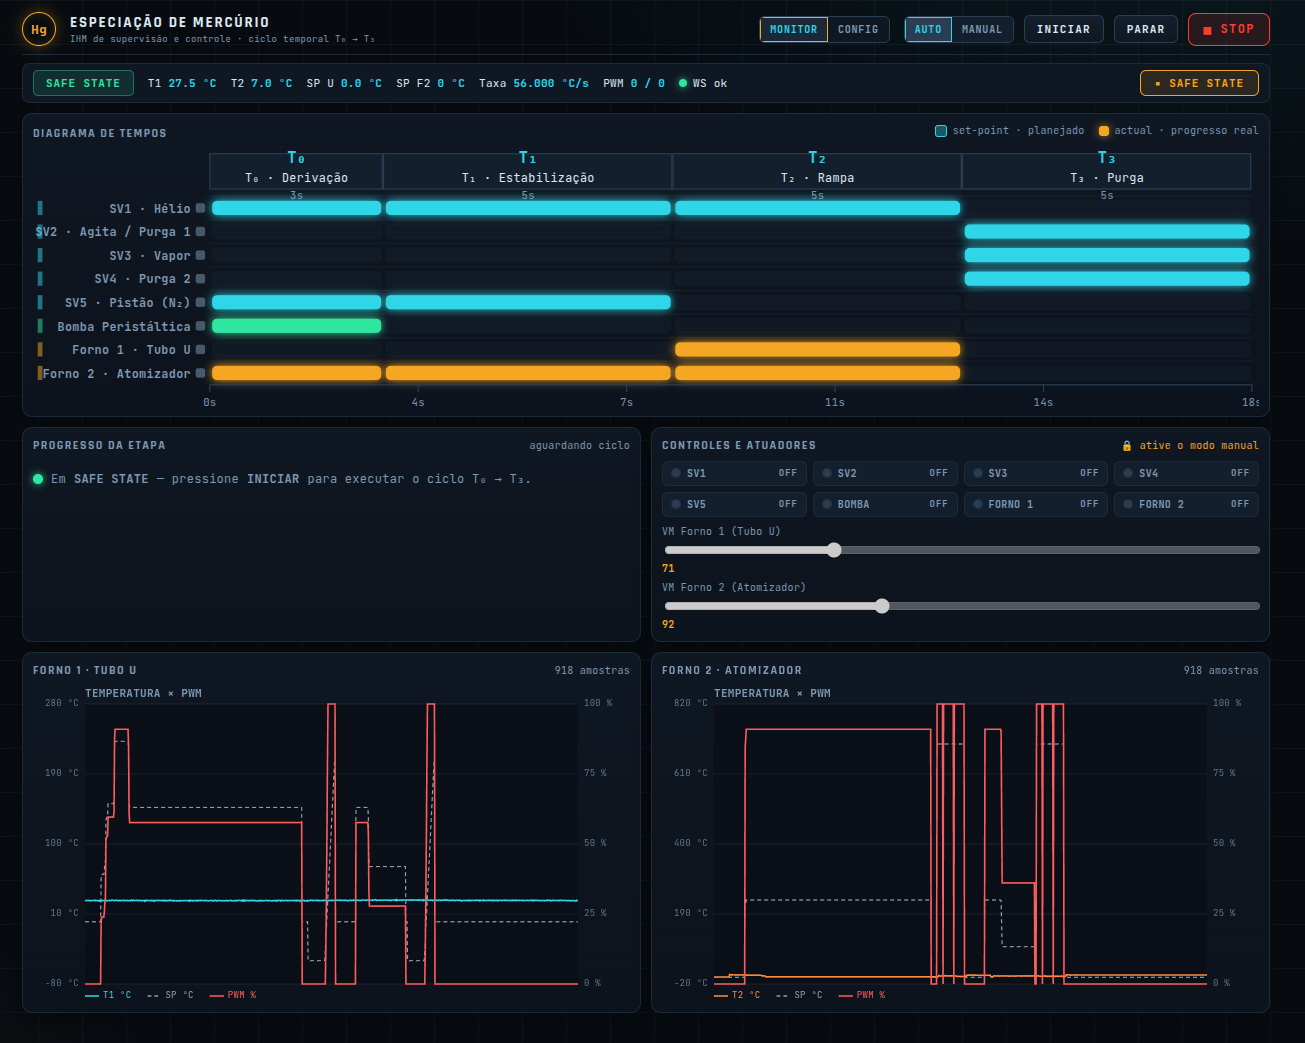
\includegraphics[width=0.92\textwidth]{frontendweb.png}
\caption{IHM Web em modo de monitoramento (Diagrama de Tempos, progresso da etapa, controles e atuadores e gr\'aficos de tend\^encia).}
\label{fig:ihm}
\par\vspace{2pt}{\footnotesize Fonte: captura de tela da IHM do projeto.}
\end{figure}

No modo autom\'atico, os controles manuais s\~ao bloqueados na interface,
evitando opera\c{c}\~ao indevida durante o ciclo; o bot\~ao de emerg\^encia
(STOP), por\'em, permanece sempre acess\'ivel e tem prioridade m\'axima,
enviando o comando de emerg\^encia ao backend e conduzindo o processo ao estado
seguro.

\section{Seguran\c{c}a e tratamento de falhas}

A estrat\'egia de seguran\c{c}a \'e composta por m\'ultiplas camadas:

\begin{enumerate}[label=\arabic*)]
  \item \textbf{Estado seguro por padr\~ao:} na inicializa\c{c}\~ao do firmware,
  todos os pinos s\~ao configurados e todas as sa\'idas s\~ao colocadas no estado
  seguro (v\'alvulas e bomba desligadas, fornos com PWM nulo e pist\~ao na
  posi\c{c}\~ao de seguran\c{c}a);
  \item \textbf{Watchdog no firmware:} desliga os fornos se nenhum pacote v\'alido
  chegar em mais de 1~s, cobrindo inclusive a desconex\~ao f\'isica do cabo USB;
  \item \textbf{Watchdog no backend:} comuta a FSM para o estado seguro se o
  \daq n\~ao responder em mais de 1~s;
  \item \textbf{Parada de emerg\^encia:} o comando de emerg\^encia \'e aceito em
  qualquer estado e tem prioridade sobre o sequenciamento;
  \item \textbf{Interlock de opera\c{c}\~ao:} no modo autom\'atico, os controles
  manuais s\~ao bloqueados, e o acionamento de um novo ciclo s\'o \'e permitido a
  partir do estado seguro.
\end{enumerate}

A combina\c{c}\~ao dessas camadas assegura que falhas de comunica\c{c}\~ao e
erros de opera\c{c}\~ao n\~ao evoluam para condi\c{c}\~oes de risco ao
equipamento (congelamento permanente do Tubo U ou sobreaquecimento dos fornos)
ou \`a seguran\c{c}a do operador.

% ======================================================================
% CAPÍTULO 6 — RESULTADOS E DISCUSSÃO
% ======================================================================
\chapter{RESULTADOS E DISCUSSÃO}

Este capítulo apresenta os resultados da validação do sistema, obtidos pela
execução das suítes de testes automatizados descritas na metodologia, e discute
esses resultados à luz dos requisitos e dos critérios de aceitação definidos. Os
valores reportados correspondem a execuções reais realizadas no ambiente de
desenvolvimento do projeto.

\section{Estratégia de validação executada}

A validação foi organizada em três frentes, conforme a camada do sistema:

\begin{itemize}
  \item \textbf{Backend (Python):} testes unitários (FSM, PID, rampa,
  persistência, enlace serial), testes da API REST e do WebSocket e testes
  funcionais de ciclo completo e de segurança, executados com o \texttt{pytest};
  \item \textbf{Firmware (\daq):} testes \emph{host-based} da biblioteca
  portável \texttt{daqcore} (parser JSON, watchdog e pulso da bomba), executados
  sem hardware no ambiente \texttt{native} do PlatformIO;
  \item \textbf{IHM Web:} testes unitários dos \emph{stores} de telemetria, de
  acionamento manual e de tema, executados com o Vitest.
\end{itemize}

A Tabela~\ref{tab:testes} consolida os resultados das execuções.

\begin{table}[htbp]
\centering
\caption{Resultado da execução das suítes de testes automatizados.}
\label{tab:testes}
\begin{tabular}{lcccc}
\toprule
\textbf{Camada} & \textbf{Ferramenta} & \textbf{Arquivos} & \textbf{Testes} & \textbf{Resultado} \\
\midrule
Backend (Python) & pytest & 8 & 40 & 40 aprovados \\
Firmware (\daq) & PlatformIO (host) & 1 & 14 & 14 aprovados \\
IHM Web & Vitest & 4 & 13 & 13 aprovados \\
\midrule
\textbf{Total} & --- & 13 & 67 & 67 aprovados \\
\bottomrule
\end{tabular}
\end{table}

\par\vspace{-2pt}{\footnotesize Fonte: execu\c{c}\~oes realizadas em 05/09/2026 no ambiente de desenvolvimento do projeto.}

\section{Testes unit\'arios e de integra\c{c}\~ao}

\subsection{Backend}

Os testes do backend cobrem os principais m\'odulos da l\'ogica de supervis\~ao:

\begin{itemize}
  \item \textbf{FSM:} valida\c{c}\~ao das transi\c{c}\~oes entre estados, da
  matriz de acionamento em cada fase e do comportamento dos eventos de parada e
  de emerg\^encia;
  \item \textbf{PID e rampa:} valida\c{c}\~ao do c\'alculo da sa\'ida do
  controlador, da satura\c{c}\~ao, do anti-windup, da taxa de aquecimento e da
  sele\c{c}\~ao das duas regi\~oes de controle da rampa (raz\~ao de taxas abaixo
  de $0\,\celsius$ e PID acima);
  \item \textbf{Persist\^encia:} valida\c{c}\~ao da escrita e leitura at\^omicas,
  da restaura\c{c}\~ao do backup e da valida\c{c}\~ao de faixas;
  \item \textbf{Enlace serial:} valida\c{c}\~ao do codec JSON, da
  serializa\c{c}\~ao/desserializa\c{c}\~ao e do tratamento de pacotes
  malformados;
  \item \textbf{API e integra\c{c}\~ao:} valida\c{c}\~ao dos endpoints de
  configura\c{c}\~ao e de comando e do fluxo de ciclo completo com simulador de
  \daq via portas seriais virtuais.
\end{itemize}

\subsection{Firmware}

Os testes do firmware (\texttt{test\_daqcore}) validam: o parser de pacotes JSON
(escrita e handshake de configura\c{c}\~ao), a rejei\c{c}\~ao de JSON inv\'alido,
a satura\c{c}\~ao do PWM, a constru\c{c}\~ao do pacote de resposta, o
comportamento do watchdog (n\~ao disparo antes do tempo limite, disparo ap\'os o
tempo limite e rearme por nova batida) e a l\'ogica de pulso da bomba (pulso nas
transi\c{c}\~oes liga/desliga e encerramento ap\'os o tempo definido).

\subsection{IHM Web}

Os testes do frontend validam a l\'ogica de assinatura e consumo da telemetria
WebSocket, o sincronismo do estado dos controles manuais com a telemetria e a
persist\^encia da prefer\^encia de tema, garantindo que os componentes reajam
corretamente aos dados recebidos.

\section{Testes funcionais do ciclo completo}

Os testes funcionais exercitam o ciclo autom\'atico $T_0 \to T_3$ com o
simulador do \daq, verificando que a FSM percorre as quatro fases na ordem
correta e que a matriz de acionamento \'e aplicada conforme o esperado em cada
fase (Tabela~\ref{tab:matriz}). A valida\c{c}\~ao confirmou que: (i) o ciclo
somente inicia a partir do estado seguro; (ii) as dura\c{c}\~oes das fases
seguem os par\^ametros configurados; e (iii) a telemetria publicada ao longo do
ciclo cont\'em o estado, o progresso da etapa e o progresso geral do ciclo,
habilitando o Diagrama de Tempos e a barra de progresso da IHM.

Adicionalmente, o roteiro de estresse de comunica\c{c}\~ao a 4~Hz, executado com
o simulador via \texttt{socat}, exercita o enlace serial de forma cont\'inua,
verificando a integridade da troca de pacotes e a estabilidade do loop de
controle ao longo do tempo.

\section{Testes de seguran\c{c}a}

Os cen\'arios de seguran\c{c}a simulam a perda de comunica\c{c}\~ao serial e
verificam as duas camadas de prote\c{c}\~ao:

\begin{itemize}
  \item \textbf{Watchdog do firmware:} quando nenhum pacote v\'alido \'e recebido
  dentro do tempo limite (1~s), o firmware comuta os atuadores para o estado
  seguro, desligando os fornos;
  \item \textbf{Watchdog do backend:} quando o \daq deixa de responder por mais
  de 1~s em uma fase ativa, o backend dispara o evento de emerg\^encia e a FSM
  retorna ao estado seguro.
\end{itemize}

Os testes confirmam que, em ambos os casos, os fornos s\~ao desligados dentro do
intervalo de seguran\c{c}a especificado ($\le 1$~s), atendendo ao crit\'erio de
aceita\c{c}\~ao de seguran\c{c}a.

\section{Discuss\~ao}

\subsection{Atendimento aos objetivos de valida\c{c}\~ao}

Os resultados obtidos indicam que a implementa\c{c}\~ao atende aos objetivos
funcionais e de seguran\c{c}a definidos na metodologia, com 67 testes aprovados
distribu\'idos pelas tr\^es camadas do sistema. Tr\^es observa\c{c}\~oes merecem
destaque:

\begin{enumerate}[label=\arabic*)]
  \item \textbf{Corre\c{c}\~ao da l\'ogica de controle:} os testes de FSM, PID e
  rampa validam matematicamente a estrat\'egia de controle mista, incluindo o
  tratamento da satura\c{c}\~ao e a sele\c{c}\~ao da regi\~ao de opera\c{c}\~ao,
  o que \'e condi\c{c}\~ao necess\'aria --- ainda que n\~ao suficiente --- para a
  qualidade da rampa em bancada;
  \item \textbf{Seguran\c{c}a por constru\c{c}\~ao:} a valida\c{c}\~ao dos
  watchdogs em ambas as camadas demonstra que o requisito de parada segura
  autom\'atica \'e atendido no n\'ivel de software, independentemente do
  hardware;
  \item \textbf{Integra\c{c}\~ao entre camadas:} os testes de ciclo completo com
  simulador confirmam a coer\^encia entre a FSM, o protocolo serial e a
  telemetria consumida pela IHM, reduzindo o risco de falhas de integra\c{c}\~ao
  quando o hardware real for conectado.
\end{enumerate}

\subsection{Compara\c{c}\~ao com os crit\'erios de aceita\c{c}\~ao}

Dos cinco crit\'erios de aceita\c{c}\~ao consolidados na
Tabela~\ref{tab:criterios}, tr\^es puderam ser verificados no ambiente de
valida\c{c}\~ao (disponibilidade da comunica\c{c}\~ao, persist\^encia e
seguran\c{c}a do watchdog) e dois dependem de medi\c{c}\~ao em bancada
(linearidade da rampa e estabilidade do Forno 2). \'E importante destacar que
esses \'ultimos s\~ao crit\'erios de \emph{desempenho t\'ermico} do processo
f\'isico e n\~ao podem ser atestados por testes de software: eles exigem a
calibra\c{c}\~ao da curva de aquecimento do Tubo U e a verifica\c{c}\~ao
experimental das curvas de temperatura, etapas de continuidade deste trabalho.

\subsection{Limita\c{c}\~oes}

A principal limita\c{c}\~ao da valida\c{c}\~ao realizada \'e a aus\^encia de
medi\c{c}\~oes em bancada com o processo f\'isico. Os testes automatizados
validam a correta execu\c{c}\~ao da l\'ogica e dos mecanismos de seguran\c{c}a,
mas n\~ao substituem a verifica\c{c}\~ao experimental da din\^amica t\'ermica.
Al\'em disso, a raz\~ao de taxas empregada na regi\~ao de malha aberta depende da
calibra\c{c}\~ao da taxa de aquecimento do sistema (curva ``Taxa $\times$ PWM''),
que deve ser medida no equipamento real; na aus\^encia desse dado, a
implementa\c{c}\~ao adota uma aproxima\c{c}\~ao que precisa ser confirmada.
Registra-se, ainda, a indefini\c{c}\~ao quanto ao circuito integrado exato de
convers\~ao do termopar (MAX6675 ou MAX31855), que n\~ao altera a l\'ogica de
controle, mas deve ser confirmada na documenta\c{c}\~ao f\'isica do equipamento.

\subsection{Implica\c{c}\~oes}

No plano t\'ecnico, os resultados demonstram a viabilidade da arquitetura
proposta para substituir o sistema legado, com vantagens de custo, flexibilidade
e seguran\c{c}a. No plano operacional, a persist\^encia dos par\^ametros e o
registro de tend\^encias criam condi\c{c}\~oes para a repetibilidade e a
auditoria do m\'etodo, requisitos valorizados em ambiente anal\'itico. A etapa de
valida\c{c}\~ao em bancada \'e o passo natural para confirmar os crit\'erios de
desempenho t\'ermico e para calibrar a rampa do Tubo U.

% ======================================================================
% CAPÍTULO 7 — CONCLUSÃO
% ======================================================================
\chapter{CONCLUSÃO}

Este capítulo retoma o problema e os objetivos propostos na introdução, sintetiza
as contribuições do trabalho, apresenta as limitações e indica direções para
trabalhos futuros.

\section{Síntese do trabalho}

Este trabalho apresentou o projeto e a implementação de um sistema de automação
e supervisão para a preparação de amostras em especiação de mercúrio, concebido
para substituir um sistema legado baseado em LabVIEW. A solução adota uma
arquitetura mestre-escravo composta por um Raspberry Pi (lógica de alto nível em
Python), um Arduino Uno (aquisição de dados em tempo real) e uma IHM Web em
React e TypeScript, integrados por um protocolo JSON a 4~Hz.

A hipótese de trabalho foi confirmada no nível de validação alcançado: a
arquitetura proposta atende aos requisitos funcionais e de segurança definidos,
proporcionando controle sequenciado do processo por máquina de estados finita,
controle PID misto da temperatura, persistência auditável dos parâmetros e
parada segura automática por watchdog duplo. A validação por testes
automatizados --- 67 testes aprovados distribuídos entre backend, firmware e IHM
Web --- demonstrou a correção da lógica de controle, a integração entre as
camadas e a efetividade dos mecanismos de segurança no nível de software.

\section{Atendimento aos objetivos}

Retomando os objetivos específicos estabelecidos no Capítulo~1:

\begin{enumerate}[label=\arabic*)]
  \item O processo foi modelado em uma FSM com os estados \texttt{SAFE},
  \texttt{T0\_DERIV} a \texttt{T3\_PURGA} e \texttt{MANUAL}, e a matriz de
  acionamento dos atuadores foi implementada e validada por testes;
  \item O controle PID misto do Tubo U --- razão de taxas abaixo de
  $0\,\celsius$ e PID em malha fechada acima --- e o controle do Forno 2 a
  $700\,\celsius$ foram implementados e verificados por testes de unidade;
  \item O protocolo JSON estruturado entre Raspberry Pi e Arduino, com handshake
  de parametrização e pacotes de escrita e leitura a 4~Hz, foi definido e
  implementado em ambas as plataformas;
  \item O firmware do DAQ foi desenvolvido com leitura de termopares via SPI,
  acionamento de atuadores (incluindo o tratamento da bomba por pulso) e
  watchdog de segurança;
  \item A IHM Web foi desenvolvida com monitoramento em tempo real, Diagrama de
  Tempos, gráficos de tendência e painéis de controle e de configuração;
  \item A persistência atômica dos parâmetros do método em JSON, com backup
  rotativo e validação de faixas, foi implementada e testada;
  \item A validação foi conduzida por testes unitários, de integração,
  funcionais e de segurança, seguindo a estratégia de desenvolvimento orientado
  a testes.
\end{enumerate}

Dessa forma, o objetivo geral --- projetar e implementar um sistema de automação
e supervisão para a preparação de amostras em especiação de mercúrio, com
parâmetros persistentes e segurança operacional --- foi alcançado no âmbito do
escopo definido.

\section{Contribuições}

As principais contribuições deste trabalho são:

\begin{itemize}
  \item a modelagem explícita e verificável do sequenciamento do processo em uma
  máquina de estados finita, com matriz de acionamento documentada;
  \item a estratégia de controle misto da rampa do Tubo U, que contorna a
  limitação de leitura do termopar na região criogênica pela razão de taxas e
  emprega PID em malha fechada na região de leitura confiável;
  \item a arquitetura mestre-escravo de baixo custo com separação entre a lógica
  de supervisão e a execução em tempo real;
  \item o protocolo de comunicação JSON aberto e legível, facilitando
  depuração, manutenção e evolução;
  \item o projeto de segurança em camadas, com estado seguro por padrão e
  watchdog duplo, suprindo uma lacuna do sistema legado;
  \item a validação sistemática por testes automatizados, conferindo
  rastreabilidade entre requisitos, implementação e resultados.
\end{itemize}

\section{Limitações}

As limitações deste trabalho decorrem, principalmente, da indisponibilidade da
bancada física durante o desenvolvimento. A validação foi realizada em ambiente
simulado; os critérios de desempenho térmico --- linearidade da rampa e
estabilidade do Forno 2 --- e a calibração da curva de aquecimento do Tubo U
permanecem pendentes de verificação experimental. Registra-se, ainda, que
questões como a identificação exata do conversor de termopar e a definição da
margem de proteção de temperatura dependem da documentação e das decisões do
responsável técnico do equipamento.

\section{Trabalhos futuros}

Como desdobramentos naturais deste trabalho, sugere-se:

\begin{enumerate}[label=\arabic*)]
  \item validar o sistema em bancada com o processo físico, calibrando a curva
  de aquecimento do Tubo U e verificando a linearidade da rampa e a estabilidade
  do Forno 2;
  \item implementar a integração automática com o detector Lumex e a exportação
  das curvas geradas (CSV/PDF) para registro e auditoria;
  \item adicionar autenticação de operadores e trilha de auditoria das ações;
  \item desenvolver um simulador de processo para treinamento de operadores;
  \item implementar a sintonização automática (auto-tune) dos controladores PID;
  \item avaliar a substitui\c{c}\~ao do bit-bang SPI por hardware SPI nativo e a
  inclus\~ao de medi\c{c}\~ao redundante de temperatura para maior robustez.
\end{enumerate}

Em síntese, o trabalho atingiu o objetivo de modernizar a automação e a
supervisão do processo de preparação de amostras para especiação de mercúrio,
entregando uma solução modular, segura e validada por testes, que estabelece uma
base sólida para a validação experimental e para a evolução contínua do sistema.


% ------------------------------ referências ---------------------------
\clearpage
\renewcommand{\bibname}{REFERÊNCIAS}
\renewcommand{\bibsection}{%
  \chapter*{\bibname}%
  \addcontentsline{toc}{chapter}{REFERÊNCIAS}}
\bibliographystyle{plain}
\bibliography{references}

% ------------------------------ apêndices -----------------------------
\appendix
% ======================================================================
% APÊNDICE A — MAPA DOS MÓDULOS DO SISTEMA
% ======================================================================
\chapter{MAPA DOS MÓDULOS DO SISTEMA}

Este apêndice consolida o mapa dos principais módulos implementados, indicando a
localização de cada componente no repositório do projeto, de modo a preservar a
rastreabilidade entre a descrição do texto e o código-fonte.

\begin{table}[htbp]
\centering
\caption{Localiza\c{c}\~ao e responsabilidade dos m\'odulos do sistema.}
\label{tab:mapa}
\footnotesize\setlength{\tabcolsep}{4pt}
\begin{tabular}{p{3.8cm}p{6.4cm}p{4.7cm}}
\toprule
\textbf{M\'odulo} & \textbf{Localiza\c{c}\~ao} & \textbf{Responsabilidade} \\
\midrule
FSM & \texttt{backend/app/fsm.py} & Estados, eventos e matriz de acionamento \\
PID & \texttt{backend/app/pid.py} & Controlador P+I com anti-windup \\
Rampa & \texttt{backend/app/ramp.py} & Rampa do Tubo U e taxa de aquecimento \\
Enlace serial & \texttt{backend/app/serial\_link.py} & Codec JSON e reconex\~ao \\
Loop de controle & \texttt{backend/app/loop.py} & Ciclo 4~Hz e watchdog do backend \\
Persist\^encia & \texttt{backend/app/config\_store.py} & Escrita at\^omica com backup \\
API e servidor & \texttt{backend/app/api.py}; \texttt{main.py} & REST, WebSocket e f\'abrica \\
Mapeamento de pinos & \texttt{firmware/src/pin\_map.h} & I/O, Safe State e pulsos \\
Driver de atuadores & \texttt{firmware/src/actuator\_driver.*} & V\'alvulas, PWM e bomba \\
Termopares & \texttt{firmware/src/thermocouple\_reader.*} & Leitura SPI (MAX6675) \\
Biblioteca \daq{} & \texttt{firmware/lib/daqcore/*} & Parser JSON, watchdog e toggle \\
IHM Web & \texttt{frontend/src/*} & Monitoramento, controle e configura\c{c}\~ao \\
\bottomrule
\end{tabular}
\par\vspace{2pt}{\footnotesize Fonte: elaborada pelo autor com base na estrutura do reposit\'orio do projeto.}
\end{table}

O reposit\'orio do projeto \'e organizado em quatro pastas principais:
\texttt{backend} (l\'ogica de supervis\~ao em Python), \texttt{firmware}
(c\'odigo do Arduino em C++, gerenciado pelo PlatformIO \cite{platformio}),
\texttt{frontend} (IHM Web em React e TypeScript \cite{react}) e \texttt{docs}
(documenta\c{c}\~ao t\'ecnica e de requisitos). A documenta\c{c}\~ao operacional
e os contratos de interface s\~ao mantidos na pr\'opria documenta\c{c}\~ao
t\'ecnica do projeto, preservando uma fonte \'unica de verdade para a
integra\c{c}\~ao entre as camadas.


\end{document}
